% !Mode:: "TeX:UTF-8"
%!TEX program  = xelatex

\documentclass[bwprint]{gmcmthesis}
%\documentclass[bwprint,fontset=fandol]{gmcmthesis} % Overleaf 等在线平台需要用这一行。
\usepackage[framemethod=TikZ]{mdframed}

\usepackage{subfig}
\usepackage{colortbl}
\usepackage{longtable}
\definecolor{color1}{rgb}{0.78,0.88,0.99}
\definecolor{color2}{rgb}{0.36,0.62,0.84}
%\definecolor{color3}{rgb}{0.8235,0.8706,0.9373}
\definecolor{color3}{rgb}{0.88,0.92,0.96}
\definecolor{color4}{rgb}{0.96,0.97,0.98}%{0.9176,0.9373,0.9686}

% 算法
\usepackage[noend]{algpseudocode}
\usepackage{algorithmicx,algorithm}
\floatname{algorithm}{算法}
\renewcommand{\algorithmicrequire}{\textbf{输入:}}
\renewcommand{\algorithmicensure}{\textbf{输出:}}

%\numberwithin{equation}{section}
%\numberwithin{figure}{section}
%\numberwithin{table}{section}


\newcommand{\red}[1]{\textcolor{red}{#1}}
\newcommand{\blue}[1]{\textcolor{blue}{#1}}



\title{WLAN组网中网络吞吐量建模}
\baominghao{24100130040} %参赛队号
\schoolname{北京邮电大学}%学校名称
\membera{沈飞} %队员A
\memberb{汪金锋} %队员B
\memberc{张睿涵} %队员C
\begin{document}

 %生成标题
 \maketitle

 %填写摘要
\begin{abstract}
    
    本文通过对WLAN网络中的接入点(AP)在不同网络环境下的行为进行建模和分析,旨在预测系统吞吐量并提出优化方案。研究内容分为三个主要部分,分别针对WLAN网络的信道接入机制、物理层速率(MCS与NSS)的选取、以及系统吞吐量的预测展开详细分析。
    
    \textbf{问题1:}信道接入分析
   
    首先,本文探讨了WLAN网络中AP之间的信道接入竞争机制。由于多个AP和STA(站点)在同一信道上通信,会产生竞争效应,影响网络的整体性能。通过对训练集中的数据分析,重点研究了AP发送数据帧序列的总时长、节点间RSSI(接收信号强度指示)以及信道接入门限等信息,建立了AP发送数据包机会关于测试基本信息的模型,该模型刻画了信道接入的时机、信道占用时间,以及由于多AP干扰带来的信道访问失败问题。通过分析这些特征信息,可以初步预测AP在复杂信道环境中的信道接入行为,为吞吐量预测奠定基础。
   
    \textbf{问题2:}MCS与NSS的选取
   
    在WLAN网络中,AP的数据传输速率通常由调制编码方案(MCS)和空间流数(NSS)决定。本文深入研究了如何根据网络中的物理层条件,如节点间的RSSI和信道质量,预测AP在数据传输中选用的MCS和NSS组合。通过对实测训练集的分析,AP在传输过程中会选择一种最优的MCS和NSS配置,该配置在AMC(自适应调制编码)算法的收敛后会保持较长时间。基于此假设,本文构建了MCS与NSS的预测模型,结合RSSI门限信息来决定AP的速率配置。虽然预测模型的精度存在一定的局限性,但通过数据中的统计信息可以获得较为稳定的速率配置。
   
    \textbf{问题3:}系统吞吐量的预测
   
    最后,基于前两问的分析结果,包括帧时长、MCS、NSS等特征,利用多层感知机(Multilayer Perceptron, MLP)预测了为WLAN网络的系统吞吐量预测模型引入的额外特征。模型的输入特征涵盖了物理层速率、信道占用时间、信道条件和干扰情况等。最后本文使用回归模型和集成学习方法对吞吐量进行预测,并通过交叉验证与超参数调优提升预测精度。研究结果可为WLAN网络的优化提供指导,通过改善MCS和NSS的选择、改善信道环境、减少AP间干扰等手段,有望提升网络吞吐量。
   在前两问的基础上,本文进一步研究了系统吞吐量的预测问题。系统吞吐量是WLAN网络性能的关键指标,受多个因素影响,如物理层速率、信道接入时长、干扰等。基于问题一中分析的信道接入时长,问题二中预测的MCS与NSS组合,以及其他基础网络测试信息,本文构建了WLAN系统吞吐量的回归预测模型。模型的输入特征包括:
   AP发送的总时长
   预测得到的MCS与NSS组合
   节点间RSSI及其门限
   信道占用情况和干扰因素
   
   在模型的构建过程中,本文采用了回归模型和集成学习方法(如随机森林,XGBoost等),本文指出,虽然MCS与NSS的预测精度较低,但仍可以通过实际统计的真实数值对模型进行调整,保证系统吞吐量预测的精确性。
   
   本文提出的吞吐量预测模型不仅为WLAN网络性能分析提供了有效的工具,还为未来的网络优化提出了切实可行的方案。通过对信道竞争机制的深入理解,可以优化AP的信道接入策略,减少多AP之间的冲突和干扰,提升整体网络的吞吐量。此外,本文的研究成果可应用于工业、教育、医疗等多种场景,通过优化WLAN网络配置,提高用户的通信质量和业务体验。
   
   总结而言,本文通过信道接入、MCS与NSS选取,以及吞吐量预测的系统性分析,成功构建了WLAN网络的性能预测框架,为未来的无线网络优化提供了理论和实践上的指导。




\keywords{WLAN系统\quad  吞吐量\quad   RSSI\quad   SINR}
\end{abstract}

\pagestyle{plain}

%目录 不推荐加
%\tableofcontents

% \section{在线使用}

% 如果你想要在 Overleaf 使用, 那么需要设置下字体
% \begin{lstlisting}[language={[latex]TeX}]
% \documentclass[bwprint,fontset=fandol]{gmcmthesis}
% \end{lstlisting}

% 由于线上平台没有隶书,只能用楷体替代了, 大家根据自己的情况来使用。



% \uwave{欢迎关注我们的微信公众号}:

% \centerline{
\includegraphics[width=5cm]{gongzhonghao1}}
\newpage
\section{问题重述}
\subsection{问题背景}
 无线局域网(Wireless Local Area Network, WLAN)以人们的业务诉求为驱动力,部署场景日益增多,在无线化办公、教育、医疗、工业制造、仓储等场景
 都有广泛应用。尽管下一代Wi-Fi7标准的峰值速率达到30Gbps,但是在例如小区、商场、学校等高密部署场景下,相邻节点
 之间覆盖范围重叠,信号干扰碰撞问题突出,使得部署带宽和数据传输速率大幅下降。为了进一步提升系统吞吐量,对WLAN系统
 的进一步优化具有重要意义。

 精准和快速的吞吐量预测时WLAN优化问题的基础问题,能够大幅度提升WLAN系统的鲁棒性和性能(吞吐量指节点单位时间内成功发送的比特
 数)。当前的一些研究通过机器学习方法,提取各节点之间的基本信息、架构信息以及节点动态位置、动态干扰等临时信息,进行训练和建模。
 但是由于研究中使用的仿真方法并不能精确反应实际部署中快速变化的信道环境、干扰以及复杂多样的业务流,其结果在真正商用中并不能达到
 预期实用价值。

 因此,为了对WLAN进行优化,在工业、教育、医疗
 等新场景中,提升用户体验,设计一种能够基于 WLAN 实测数据,分析 WLAN 网络拓扑、节点间 RSSI、信道接
 入机制、干扰等因素对 WLAN 数据发送、速率的影响,进一步地,对 WLAN 系统吞吐量
 进行精确预测的模型具有重要研究意义。
 \subsection{问题描述}
 基于上述研究背景,题目提供了WLAN组网场景下的实测数据,数据集提供了包括测试基本信息,以及测试中收集的数据帧相关统计信息,
 围绕WLAN组网中网络吞吐量建模,提出以下问题:

 \textbf{问题1:}
 根据附件WLAN网络实测训练集中所提供的网络拓扑、业务流量、门限、节点间RSSI的测试基本信息,分析其中各参数对
 AP发送机会的影响,并给出影响性强弱的顺序。通过训练的模型,预测每个AP的发送机会,即发送数据帧序列的总时长(seq\_time),并通过测试集 test\_set\_1\_2ap和test\_set\_1\_3ap(仅提供模型输入信息)预测AP发送数据帧序列的总时长。可按照同频AP个数分类分析和分别建模,也可统一分析和建模。

 \textbf{问题2:}
 根据附件提供的实测训练集中的测试基本信息,特别是节点间RSSI信息和门限信息,结合问题1中对AP发送机会的分析,对测试中AP发送数据选用最多次数的(MCS, NSS)进行建模
 ,并通过测试集(仅提供模型输入信息)预测(MCS, NSS)。
 
 \textbf{问题3:}
 结合问题1和问题2的分析,对系统吞吐量进行建模,并通过测试集test\_set\_1\_2ap和test\_set\_1\_3ap预测网络吞吐量。
 可按照同频AP个数分类建模,也可统一建模。本问题允许采用实测中统计的数据帧真实(MCS, NSS)作为模型输入变量。

 
 \newpage
 \section{模型假设与符号说明}
    \subsection{模型假设}
 1.	假设任意两AP之间在互相影响的效力上具有对等地位,对各自有同样的干扰;
 
 2.假设基站位置信息对AP之间干扰的影响,仅通过RSSI值来体现;
 
 3.假设在传输方式为同步的时候,环境底噪为-100dbm;
  
 \subsection{符号说明}

 
 \begin{table}[htp!]
 \centering
 \renewcommand\arraystretch{1.2} %定义表格高度
 \newcolumntype{L}{>{\quad}X}
 \newcolumntype{P}[1]{>{\centering\arraybackslash}p{#1}}
 \newcolumntype{C}{>{\centering \arraybackslash}X}
 \newcolumntype{R}{>{\raggedright \arraybackslash}X}
 \begin{tabularx}{0.9\textwidth}{|P{2cm}|L|}
   \hline %\toprule
   符号    &   \quad 意义 \\
   \hline %\midrule      
   %\rowcolor[gray]{0.90}
   $ T_{\text{seq\_time}} $        &  数据帧发送总时长    \\
   \hline
   $ T_{\text{PPDU}} $        &  发送一个数据包的平均时长    \\
   \hline
   
   $ L_{\text{PPDU}} $        &   一个PPDU数据包的长度    \\
   \hline
   $ L_{\text{MPDU}} $        &   一个MPDU数据包的长度    \\
   \hline
 
   $ L_{\text{MSDU}} $        &   一个MSDU数据包的长度    \\
   \hline
   
   $ N_{\text{AMPDU}} $        &    一次AMPDU聚合过程中使用的MPDU数据包个数   \\
   \hline
   $ N_{\text{AMSDU}} $        &    一次AMSDU聚合过程中使用的MSDU数据包个数   \\
   \hline
   $ \text{PER} $        &  丢包率    \\
   \hline
   $ \text{Throughput} $        &  吞吐量    \\ 
   \hline %\bottomrule
   $ \text{Trans} $        &   传输方式    \\
   \hline
%    $ i $        &       \\
%    \hline
%    $ i $        &       \\
%    \hline
 \end{tabularx}
 \end{table}
 
 
 %\begin{tabularx}{\textwidth-18pt}{XXX}
 %\hline
 %Input & Output& Action return \\
 %\hline
 %DNF &  simulation & jsp\\
 %\hline
 %\end{tabularx}

%  \newpage
% \section{问题分析}
% 主要是表达对题目的理解,特别是对附件的数据进行必要分析、描述(一般都有数据附件),这是需要提到分析数据的方法、理由。如果有多个小问题,可以对每个小问题进行分别分析。
% (假设有2个问题)



% \subsection{问题1的分析}

% 对问题1研究的意义的分析。

% 问题1属于。。。。。数学问题,对于解决此类问题一般数学方法的分析。

% 对附件中所给数据特点的分析。

% 对问题1所要求的结果进行分析。

% 由于以上原因,我们可以将首先建立一个。。。。。。的数学模型I,然后将建立一个。。。。。。。的模型II,。。。。。。。。。。对结果分别进行预测,并将结果进行比较.


% \subsection{问题2的分析}


% 对问题2研究的意义的分析。



\newpage
\section{基本原理}
\subsection{接入机制}
WLAN中工作在同一信道的各节点共享信道,节点通过载波侦听多址接入/退避的机制避免冲突。接入过程可分为以下3个步骤: 
\setlist[enumerate]{label=(\arabic*),left=1em} % 设置item之间的间距为1.5em,并整体缩进
\begin{enumerate}
    \item 信道可用评估(Clear Channel Assessment,CCA):节点有数据要发送时,首先对工作信道进行固定时长的载波侦听,这个固定时长被称为分布式协调帧间距(Distributed Coordination Function Inter-frame Space, DIFS)。如果DIFS时段内接收到的信号强度RSSI低于CCA门限,判断信道为空闲,否则判断信道为繁忙。
    \item 随机回退:判断信道为空闲时,为避免节点间碰撞,每个节点根据其竞争窗口(Contention Window, CW),从[0, CW–1]的整数均匀分布选取一个随机整数作为回退数,将其乘以时隙slotTime(9μs),称为随机回退时段。如果信道在随机回退时段保持空闲,则节点开始一次数据传输。如果期间信道变繁忙,节点将暂停回退,直到信道重新在DIFS内空闲,再继续前面的回退。随机回退采用二进制指数退避算法确定。
    \item 数据传输:回退到0的节点发送一个数据帧,接收节点在成功接收到数据之后等待短帧帧间距(Short Inter-frame Space, SIFS)16μs,回复确认帧(Acknowledgement, ACK)32μs。
\end{enumerate}
\subsection{CCA门限}
WLAN有两层协议栈,即物理(Physical, PHY)层和媒体接入控制(Medium Access Control, MAC)层。数据字段首先在MAC层封装MAC头,携带源MAC地址和目的MAC地址,接着在PHY层封装上PHY头,用于调制和解码,形成一个完整的Wi-Fi帧被发送出去。信道中传输的数据可以被一定区域内的任何其他节点接收,节点首先对PHY头解码,将解封装的数据帧上送到MAC层,节点通过MAC头携带的目的地址识别发送给自己的数据。AP通常配8根不同角度的天线接收信号,所有天线接收RSSI的和用于解码。
	WLAN引入包检测(Packet Detection, PD)门限和能量检测(Energy Detection, ED)门限这两个CCA门限,典型值分别是–82dBm和–62dBm。若节点PHY层接收机检测到完整的数据包的PHY头的前导(Preamble),则判定为Wi-Fi报文,采用PD门限;若未检测到Preamble,判定为非Wi-Fi报文,则采用ED门限判断信道忙闲。
AP通常配8根不同角度的天线接收信号,各天线所接收RSSI的和就是所接收信号的RSSI。然而,在进行PD和ED门限判决时,仅采用各天线所接收RSSI中的最大值。

\subsection{NAV机制}

	为保障低延时等高优先级业务,WLAN支持在MAC头携带网络分配矢量(Network Allocator Vector, NAV)字段,指示其它节点在该NAV时段内静默来为自己清空信道。NAV时段为该节点从发送数据帧到接收完ACK的时长。一个节点若处于其它节点指示的NAV静默期,则不竞争信道。在组网中,当AP PHY层接收到来自相邻BSS的数据帧时,若RSSI低于NAV门限(通常为–82dBm),则停止接收,直接丢弃;若RSSI高于NAV门限,则完成接收,并将其上送到MAC层,更新MAC头中携带的NAV时段。关于信道忙闲按CCA门限判断并结合静默期决定。AP采用各天线所接收RSSI的平均值用于NAV门限判决。

\subsection{随机回退}
	
随机回退采用二进制指数退避算法确定回退时间。CW的初始值为CWmin,不同节点的CWmin可以相同,也可以不同,每次数据传输失败后进行重传时,CW翻倍。如果CW达到了CWmax,则保持此值,直到被重置为止。每次数据传输成功时CW重置,开始下一个数据帧的回退。若传输连续失败,重传次数达到r后,数据帧被丢弃,CW重置传输下一个数据帧。可见,重传r次时,无论成功还是失败,CW都会重置。

附图\ref{pho:huitui}中的一次传输(Tx,transmission)包含了发送一个数据包和接收一个ACK,一次collision包含了发送一个数据包和等待ACKTimeout时长。帧序列如附图2所示,一个数据帧包括PHY头、MAC头和有效载荷payload,ACK时长为32μs,ACKTimeout为53μs。为减少冲突,AP采用RTS-CTS模式发送数据,即发送节点先发送一个请求发送(Request to Send, RTS)帧,收到的节点回复一个允许发送(Clear to Send, CTS)帧,RTS和CTS的MAC头中携带NAV,通过该方式通知发送节点和接收节点的通信范围内的其他节点在此期间静默。RTS和CTS是短帧,时长32μs,RTS或CTS碰撞,相比数据帧碰撞,可避免信道浪费。RTS-CTS模式下的帧序列如图\ref{pho:rtscts}所示。
\begin{figure}[!htbp]
    \centering
    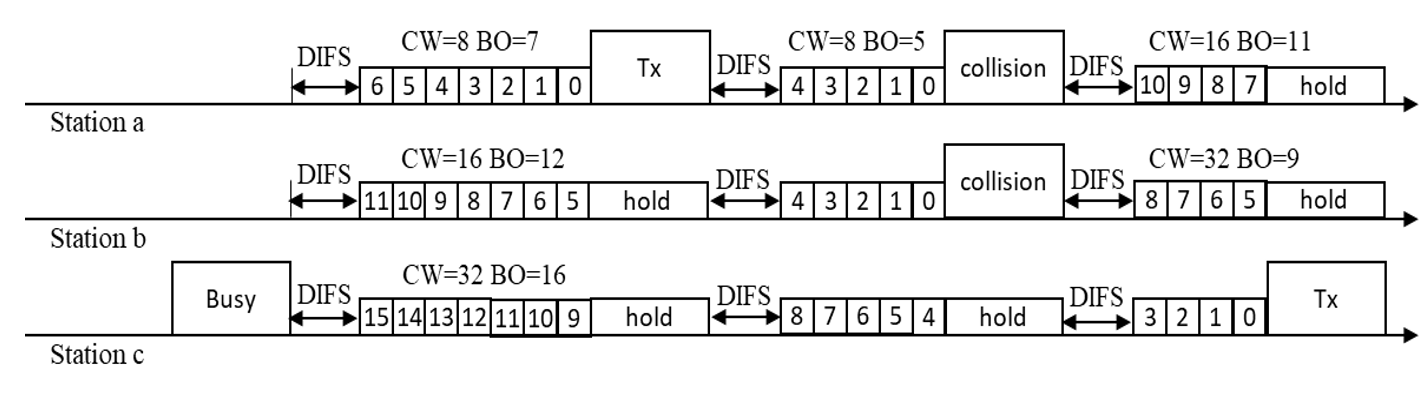
\includegraphics[scale=0.65]{huitui.png}
    \caption{\centering 二进制指数退避过程}
    \label{pho:huitui}
\end{figure}
\begin{figure}[!htbp]
    \centering
    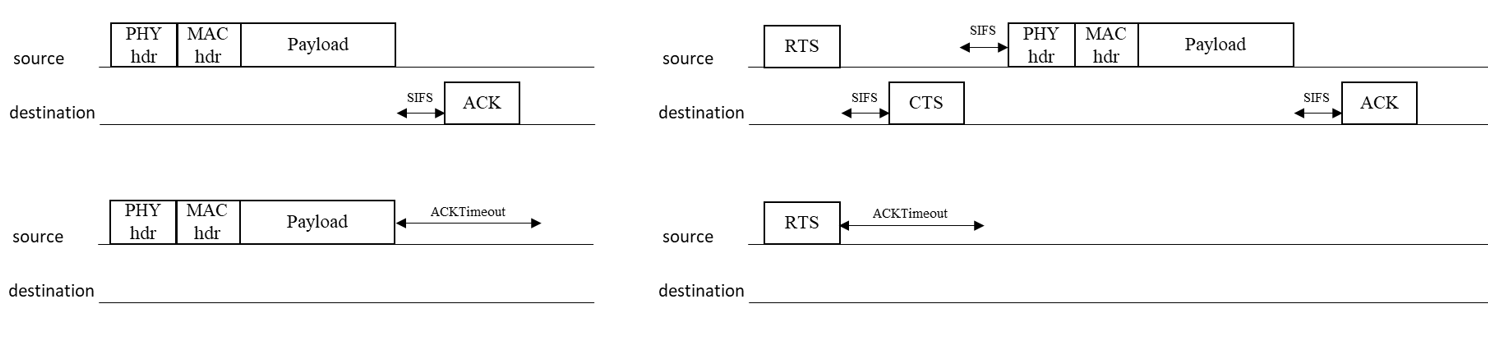
\includegraphics[scale=0.65]{rtscts.png}
    \caption{\centering 数据帧序列和RTS-CTS模式下发送成功发送失败的帧序列}
    \label{pho:rtscts}
\end{figure}

\subsection{聚合}
为了提升发送小包的效率,协议允许通过聚合一次发送多个具有相同目的地址的数据包。来自网络上层(如以太网逻辑链路层LLC层),具有相同接收地址的同服务类别的MAC服务数据单元(MAC Service Data Unit, MSDU),可以在MAC层顶端被拼接起来,加上一个共同的MAC头,封装成一个MAC协议数据单元(MAC Protocol Service Data Unit, MPDU),这个过程叫作聚合MSDU(Aggregated MPDU , AMSDU)。组装好的MPDU在MAC层底端被聚合起来,每个MPDU前加一个短分隔符,随后聚合成为一个PHY协议数据单元(PHY Protocol Data Unit, PPDU)送给PHY层。每次发送数据时,缓存里有包则聚,遵循$N_{\text{AMSDU}}$个数最多为7,$N_{\text{AMPDU}}$个数最多为21,同时,一个PPDU时长不超过4.5ms。

在进行聚合时,由于聚合的子MSDU之间,及子MPDU之间需要插入冗余字段,实际一个PPDU传输时长里,仅MSDU的总字节数是有效传输数据,进行吞吐量计算时才被计入,因此,AMS
DU和AMPDU聚合的准确评估对吞吐量预测也有影响。如附图3(a)所示,应用层报文payload长度为1420 Bytes,包含40 Bytes长的IP协议头和1380 Bytes长的有效载荷。经过以
太网有线网到达Wi-Fi的MAC层后,不聚合,加上8 Bytes的LLC层(以太网逻辑链路层)头,封装上30 Bytes的MAC头(802.11 header),形成一个MPDU。如\ref{pho:juhe}所示,缓
存里包增多时,进行聚合,MSDU之间插入0-3字节的填充字节进行4字节对齐,一个MPDU中的MSDU共用一个30 Bytes的MAC头。MPDU进行聚合时,前面加上分隔符delimiter,再进行4字节对齐,一个PPDU封装一个PHY头。

\begin{figure}[!htbp]
    \centering
    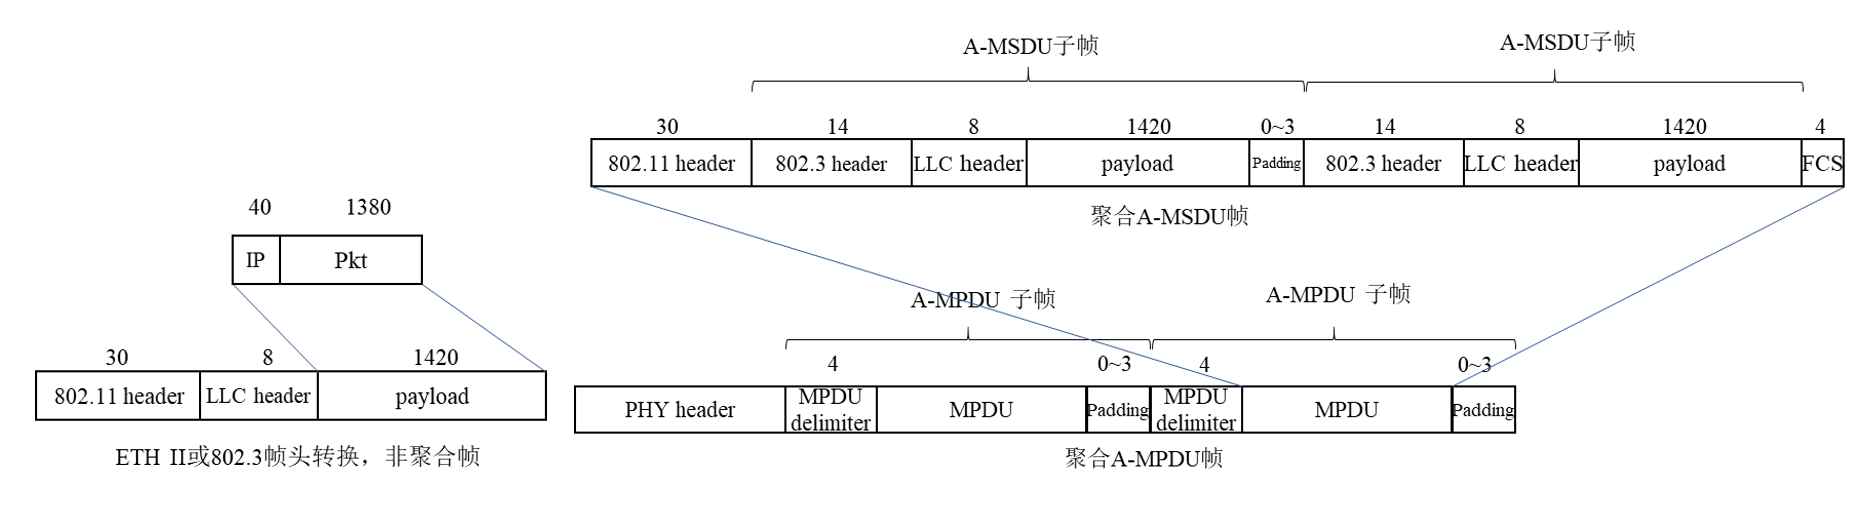
\includegraphics[scale=0.5]{juhe.png}
    \caption{\centering (a)以太网帧不聚合  (b)AMSDU聚合和AMPDU聚合}
    \label{pho:juhe}
\end{figure}
\subsection{传输方式}
当两个节点间的RSSI>ED时,一个节点传输数据时,另一节点检测信道为繁忙,称两个节点能“听”到。那么多数情况下二者的数据传输将交替进行,只在偶然同时回退到0时同时开始数据传输。节点同时发送数据时产生碰撞,可能导致传输失败。这种在节点间可侦听情况下发生的传输称为同步传输,包括交替进行和同时发生的传输。

WLAN实际部署中,受覆盖范围和可用信道数约束,工作在相同信道的同频AP间RSSI大多处于[PD, ED]区间,一个区域内同频AP数量通常为3~5个。受
业务类型影响,包长差异较大,如\ref{pho:yibu}所示,在某次同步传输过程中,先结束传输的AP2进行CCA时,由于已经错过侦听AP1的Preamble,将采用ED作
为CCA门限,从而判定信道为空闲,在回退到0时开始一次新的传输。称为异步传输。若AP1结束传输时,AP2的第二次传输已开始,则AP1同样原因可能会开始第二次传输,那么两个AP可能进入长时间的异步传输状态。

\begin{figure}[!htbp]
    \centering
    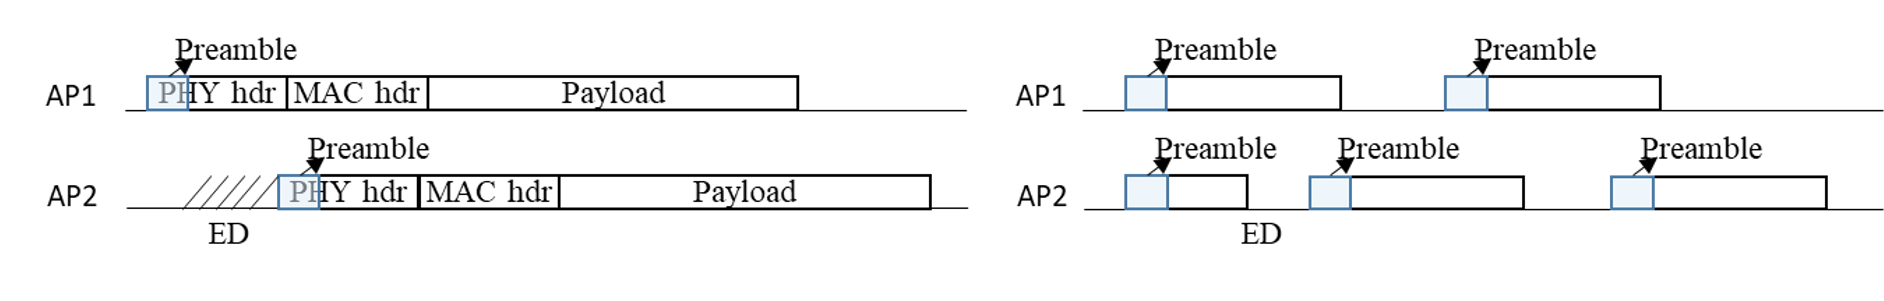
\includegraphics[scale=0.45]{yibu.png}
    \caption{\centering 一次异步传输和异步传输状态示意图}
    \label{pho:yibu}
\end{figure}
\subsection{自适应调制编码算法}
发送数据的PHY层速率(PHY Rate)由调制编码方案(Modulation and Coding Scheme, MCS)和空间流数(Number of Spatial Stream, NSS)表征,一
组(MCS, NSS)对应一个PHY Rate(见4.2节)。MCS和NSS越高,发送时携带的有效比特数越多,即PHY Rate越高。节点的PHY层对信号进行解调时,要求一定
的SINR,其SINR越高,可支持成功解调的MCS和NSS越高。WLAN采用经典的自适应调制解调(Adaptive Modulation and Coding, AMC)算法,根据信道条件
动态调整发送数据使用的(MCS, NSS)。具体地,初始化时采用默认值(如MCS6, NSS2)发送数据,并持续统计和更新丢包率(Packet Error Rate, PER)。
当PER高于一定阈值时,代表当前SINR下,以该(MCS, NSS)发送数据的解调成功率低,需要降低MCS和NSS;否则提高MCS和NSS。AMC算法自适应寻找最优的
PHY Rate发送数据,使得吞吐量最大。
\newpage
\section{问题一的分析与求解}

\subsection{问题分析}
\subsubsection{问题简述}
问题一主要研究AP发送的机会,旨在探索WLAN网络中的节点在测试场景下发送数据包的机会,即发送数据帧列的总时长(seq\_time),并构建预测模型,该问题包括两个子问题:

(1) 分析测试基本信息中各参数对seq\_time的影响并排序:

首先,基于训练集中training\_set\_2ap\_loc0\_nav82等13个数据表,对同频AP个数为2和同频AP个数为3的场景分别进行建模分析。对于每一种同频AP类型,研究表中所提供的网络拓扑、业务流量、门限、节点间RSSI的测试基本信息,分析其中各参数对AP发送机会的影响,即对seq\_time数据值的影响,并根据其影响性强弱给出重要性排序。

(2)构建模型预测每个AP的seq\_time:

根据训练集中training\_set\_2ap\_loc0\_nav82等13个数据表,分别对同频AP个数为2和同频AP个数为3构建模型预测测试集test\_set\_1\_2ap和test\_set\_1\_3ap中AP发送数据帧序列的总时长,然后将模型应用于测试集,给出测试集中seq\_time的预测值。 

通过解决问题一的两个子问题,我们将更好地了解哪些因素能够影响AP发送数据的机会,并能够进一步研究各参数对WLAN网络吞吐量的影响。这对于无线局域网系统的进一步优化具有重要意义。



\subsubsection{机制分析}
根据题目,在节点间RSSI、信道竞争接入机制、CCA门限、NAV机制等共同影响下,节点以一定的概率发送数据。故想要准确预测AP发送数据的机会,需要分别考虑上述各因素影响与综合影响,本节具体分析论述了其影响机制与运行方式。

\textbf{(1)传输方式}

节点之间的接收信号强度(Received Signal Strength Indication, RSSI)不仅体现了节点间的位置信息,还将与CCA、NAV机制共同决定节点能否争夺到信道和发出数据包。根据两节点能否互“听“,以及NAV机制是否有效,节点间的传输方式分为了同步传输、异步传输以及同步异步混合传输。

% 分析各节点之间的RSSI信息和门限信息,可以得出在WLAN信道争夺机制下,AP可能处于如下三种传输方式:

\textbf{1、同步传输:}此时AP间RSSI\_MAX>PD且RSSI\_MEAN>NAV,两AP之间互听,交替抢到信道,偶然同时发送,且NAV生效。STA接受数据时干扰主要来自环境底噪。

\textbf{2、异步传输:}此时AP间RSSI\_MAX<PD且RSSI\_MEAN<NAV,两AP之间不互听,邻区干扰小,同时进行数据发送,NAV不生效。此时STA接收数据时可能受到较小的邻区干扰和环境底噪。

\textbf{3、宏观上同步与异步传输混合:}此时两个AP的RSSI\_MAX>PD且RSSI\_MEAN<NAV,两AP之间互听,邻区干扰大,NAV不生效。当传输中出现由于错过Preamble时,无法利用NAV更新通知其他AP,导致异步传输。此时STA接收数据时受到的干扰根据具体处于的传输方式决定。

% 根据各节点间RSSI信息处于门限区间,计算得出对应SINR值,以预测对应的(MCS, NSS)。

\textbf{同步传输方式}的优点是各AP在预定时隙内传输,避免了信道竞争和冲突,保证了公平性和确定的传输时机,并减少了干扰,即使SINR较低的AP也可以获得稳定的传输时机。但其缺点在于固定时隙可能造成资源浪费,且对负载变化的灵活性较差,导致潜在的吞吐量瓶颈。如果负载不均衡,某些AP可能会浪费时隙资源。

\textbf{异步传输方式}的优点是灵活性高,AP可以随时尝试传输,动态利用信道资源,适应负载变化。当信道负载较低时,异步传输方式更有效率。然而,其缺点是信道竞争可能导致碰撞、延迟和不公平分配,对于SINR较低的AP,可能因竞争失败而传输机会减少。尤其在高密度环境中容易出现干扰和“捕获效应”,即较强的AP总是比较弱的AP占据更多的信道资源。

\textbf{(2)信干噪比(SINR)}

SINR是衡量信号质量的重要指标,其值越高,表示信号质量越好,节点间的传输效果越好。因此,我们认为节点所处环境的SINR值对于节点发送数据的机会有着重要的影响。

第(1)节中所分出的同步和异步\textbf{传输方式},导致AP能收到不同类型的干扰,使得计算SINR值的方式不同。在同步传输情况下,干扰仅包括环境底噪,而在异步传输情况下, STA 接收数据时还可能受到邻区AP的干扰。
除了传输方式外,我们发现,不同的\textbf{同频AP个数}也会导致SINR值的计算方式不同。在同频AP个数为2的场景下,AP仅需要考虑另一相邻AP的干扰,而在在同频AP个数为3的场景下,各AP均需综合考虑另外两个AP的干扰。
特别是在异步传输场景下,由于STA的传输受到邻区干扰,这一影响尤为明显。为此,我们调研了如何在3AP场景下叠加两个不同干扰源的方法,以表征其对信干噪比SINR的影响。

据调研\cite{rn1},接收信号强度指示(RSSI)可以通过多种方式计算,常见的计算方式包括线性功率值和对数功率值。不同的方式可以结合叠加使用来获得不同情境下的总接收信号强度。

1. \textbf{线性功率值}

RSSI 可以直接用功率值来表示,通常以瓦特(W)或毫瓦(mW)为单位。多个信号的线性功率值可以通过直接加和来叠加:
\[
P_{\text{total}} = P_1 + P_2 + \cdots + P_n
\]
其中 $P_i$ 表示每个信号的功率值。

2. \textbf{对数功率值}

在对数尺度下,如以分贝(dB)为单位表示 RSSI,信号强度的叠加需要将对数值转换回线性功率值,再进行加和:
\[
P_{\text{total}} = 10 \log_{10} \left(10^{P_1/10} + 10^{P_2/10} + \cdots + 10^{P_n/10}\right)
\]


考虑到RSSI具有上述两种不同的叠加方法,在计算同频AP个数为3的场景中的邻区干扰时,我们使用对数方法进行信号强度叠加,随后使用线性方法计算关联AP到该STA的RSSI与邻区AP到该STA的RSSI之差。
另外,通过简单观察训练集中各接收到RSSI参数的取值大小,发现其在测试中出现的可能范围于-98dBm至-29dBm之间,我们规定$RSSI_{noise}=-100dBm$为环境噪声强度。

综上,结合传输方式和同频AP个数两个因素,我们使用不同方法对SINR进行计算,使用'+','-'号表示线性叠加,使用 $ \oplus $ 号表示对数叠加。
具体计算公式如表\ref{tb:sinr}:

\begin{table}[htp!]
    \centering
    
    \begin{tabular}{|l|l|l|}
      \hline %\toprule
      同频AP个数    &   同步       &    异步 \\
      \hline %\midrule      
      %\rowcolor[gray]{0.90}
      2       &  $RSSI_{self\_ap} - RSSI_{noise}$     &   $RSSI_{self\_ap} - RSSI_{other\_ap}$\\
      \hline
      3        &  $RSSI_{self\_ap} - RSSI_{noise}$    & $RSSI_{self\_ap} - (RSSI_{other\_ap1} \oplus RSSI_{other\_ap2})$ \\
      \hline
      
    \end{tabular}
    \vspace{0.5cm}
    \caption{STA的SINR计算方法}
      \label{tb:sinr}
    \end{table}
其中,$RSSI_{self\_ap}$ 表示STA接收到的自身AP的信号强度,$RSSI_{other\_ap}$ 表示STA接收到的邻区AP的信号强度,$RSSI_{noise}$ 表示环境噪声强度。
% 通过简单观察训练集中各接收到RSSI参数的取值大小,发现其在测试中出现的可能范围于-98dBm至-29dBm之间,结合文中提到的CCA门限以及测试中出现的两种NAV门限,
% 某一AP节点在某一时刻根据接入机制对信道忙闲判断如下(对RSSI取值范围):

%  1. $ [ -100,NAV ) $:信道空闲。

%  2. $ [ NAV,PD ) $:若未侦测到RTS,信道空闲,否则繁忙。

%  3. $ [ PD,ED ) $:若未侦测到RTS,且未接收到Preamble,则信道空闲,否则信道繁忙。

%  4. $ [ ED,-20 ) $:信道繁忙。
    

% \begin{figure}[!htbp]
%     \centering
%     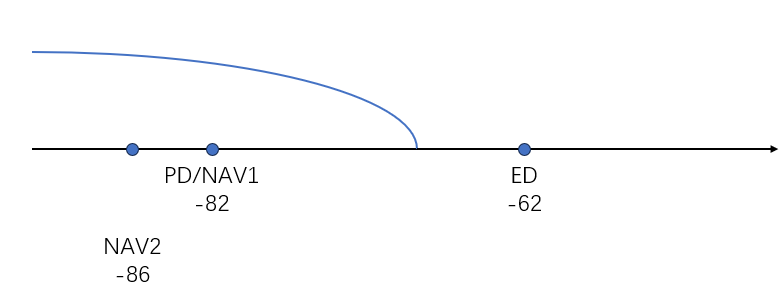
\includegraphics[scale=0.8]{menxian.png}
%     \caption{\centering CCA门限、NAV门限示意图 \quad 单位(dBm)}
%     \label{pho:menxian}
% \end{figure}

\textbf{(3)总结:}

a)RSSI作为题目给定的重要特征,体现了节点接收到来自其他拓扑中节点的信号强度。经过分析,该特征由于经过去底噪处理,时序特征较弱,且在测试期间波动不明显。
因此,我们在本题中考虑将RSSI序列用于判断节点接受的信号强度所处CAA和NAV门限区间,随后,对RSSI序列求平均,用单值替代,作为节点间的定值特征。

b)当节点接受到的RSSI较小时,即其他节点信号影响较小时,AP根据对信道忙闲的判断更大可能性为空闲,并发送数据。尽管此时仍有随即回退机制的限制,但可以推断的是,此时
AP发送数据的机会更大,并导致更长的seq\_time。相反,当节点接受到的RSSI较大时,其他节点信号影响较大,此时CCA机制和NAV机制生效的概率更高,节点需要遵守接入机制,
在预定时隙内传输,与相邻节点共用信道资源,具有有限的发送数据的机会,即seq\_time较小。因此,我们可以根据对AP所听到的RSSI强弱,判断其所处的门限区间,以进一步根据其传输方式进行分类,用于本题模型预测。

c)信干噪比(SINR)在无线通信中对AP(接入点)发送机会的影响,可以理解为SINR决定了每个AP在竞争信道时的胜率以及发送数据帧的效率。具体来说,SINR越高,意味着信号强度相对于干扰和噪声的比例越大,数据
传输的成功率越高,信道的利用率也会相应增加。然而,在WLAN网络环境中,环境噪声和邻区干扰等因素都会对SINR产生影响,随着拓扑中同频AP个数的增加,邻区干扰进一步加剧了这种影响。针对不同因素环境,
采用不同的SINR的计算方式,能够更精确地模拟测试中节点间信号干扰情况,进而更好地预测AP发送数据的机会。

综上所述,我们认为节点的RSSI信息、传输方式、节点SINR值以及门限值对预测AP的发送机会都具有一定影响。对AP发送机会的预测可表示为:
$$T_{\text{seq\_time}}=f(RSSI_{*},Trans,SINR_{sta},pd,ed,nav)$$
其中,$RSSI_{*}$表示各类RSSI信息,$Trans$表示传输方式,$SINR_{sta}$表示信干噪比,$pd,ed,nav$表示门限信息。



\subsubsection{求解思路}
针对上述问题,提出如下求解思路:

由题目可知,WLAN部署后,节点基于信道竞争接入机制进行CCA和随机回退,并发送数据。在节点间RSSI、信道竞争接入机制、CCA门限、NAV机制等共同影响下,节点以一定的概率发送数据。
因此,节点在某一功率下的某一时刻听到的\textbf{RSSI处于什么范围(是否超过门限)},会使得节点因此选择传输、等待(DIFS/回退)或静默,乃至导致可能的测试组内的传输方式(同步/异步),这一
机制能够很大程度上影响对节点数据帧发送时长的预测,因此除了使用训练集给定的参数外,我们还需要从这些给定数据中挖掘对应新特征表示节点状态以更好地进行预测。
问题一的求解思路如下图\ref{pho:wenti1}:
\begin{figure}[!htbp]
    \centering
    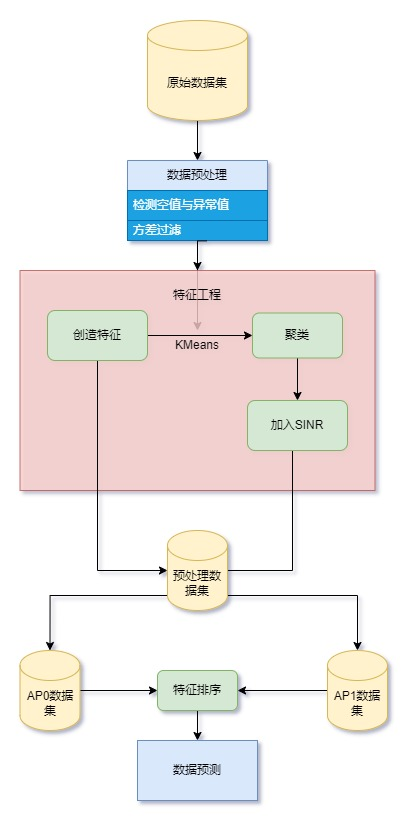
\includegraphics[scale=0.5]{wenti1.jpg}
    \caption{\centering 问题一思路示意图}
    \label{pho:wenti1}
\end{figure}

\subsection{问题求解}
\subsubsection{数据处理}
针对所提供的网络拓扑、业务流量、门限、节点间 RSSI 的测试基本信息包括共35个可选特征变量,我们进行预处理,进行以下步骤操作。

\textbf{(1)数据清洗},我们将相同同频AP个数的所有训练表合并为一个主表,对于表中观测到的异常空值,和异常数值(例如在training\_set\_3ap\_loc30\_nav86中部分列数据为空, 以及training\_set\_2ap\_loc2\_nav82最后两行的数据与其他数据相比明显异常,数据与表头内容对不上),对此处理为删除整行数据避免对分析结果的影响。

\textbf{(2)方差过滤},进行部分特征变量的移除,这些变量部分是常量(即在所有数据中保持不变),部分可以以行数奇偶性为隐藏属性表示,部分只是固有属性根据经验判断与因变量seq\_time无关。删除变量包括:test\_dur、loc\_id、pkt\_len、bss\_id、ap\_name、ap\_mac、ap\_id、pd、ed、sta\_mac、sta\_id共11个变量。

\textbf{(3)特征创造}。a.题目中提到AP传输方式对AP发送时长具有直接影响,考虑到pd,ed表现为信道传输门限,它们决定了AP的CCA机制,进而导致不同的可能传输机制,因此我们采用差值变量,以概率形式表示在某一时间点AP的传输方式可能性。变换公式如下:
\begin{align}
    pro\_pd=\frac{num_{from\_ap\_max\_rssi\_gt\_pd}}{num_{from\_ap\_rssi}}\\
    \nonumber\\
    pro\_ed=\frac{num_{from\_ap\_max\_rssi\_gt\_ed}}{num_{from\_ap\_rssi}}\\
    \nonumber\\
    pro\_nav=\frac{num_{from\_ap\_mean\_rssi\_gt\_nav}}{num_{from\_ap\_rssi}}
    \end{align}
    $num_{from\_ap\_max\_rssi\_gt\_pd}$表示在某一时间点AP听到的RSSI大于PD门限的次数,$num_{from\_ap\_rssi}$表示在测试期间AP听到的RSSI的总次数。同理可得$pro\_ed$,$pro\_nav$。
b.还引入了SINR,考虑了STA接收数据时可能受到的干扰。

\textbf{(4)聚类分析}。根据(3)中创造的三个特征变量(在 3AP 情况是两组共 6 个):pro\_pd,pro\_ed,pro\_nav,分别表示了某 AP 在一
次测试期间接收到来自其他组内 AP 的 RSSI 高于 PD、ED、NAV 门限的频率,这一组数
据体现了此次传输中各测量时刻该 AP 所接受到的 RSSI 数值所分布范围,以此近似表示
该 AP 进行对应接入操作的概率。
由于新特征呈现连续性,取值处于$[0,1]$之间,且具有不
均匀性,为了在进行门限区间分类时使用准确的阈值,我们采用 K-means 聚类辅助分析:

\textbf{K-means}是一种基于划分的无监督学习算法,旨在将数据点划分为
K个簇(cluster),使得簇内数据点的相似度尽可能高,而不同簇之间的差异尽可能大。其核心思想是通过迭代优化,将数
据点分配给最近的簇中心(centroid)。K-means适用于聚类分析,具有效率高、快速收敛的特点,适合快速给出可视化聚类效果,辅助进行本题的RSSI状态分析。

通过肘部图以及轮廓系数共同推断(图\ref{pho:julei1}),分类分成三簇,符合上文机制分析中对AP传输方式的推断。

\begin{figure}[!htbp]
    \centering
    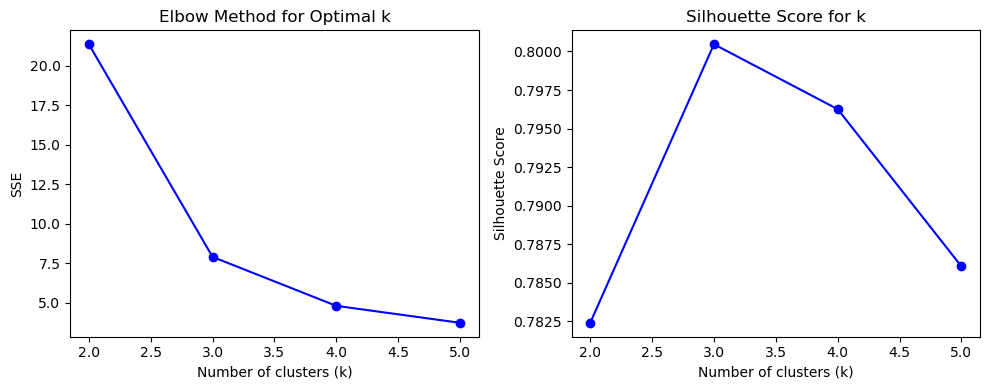
\includegraphics[scale=0.8]{julei1.png}
    \caption{\centering 肘部图(左)以及轮廓系数(右)}
    \label{pho:julei1}
\end{figure}

聚类结果如下图\ref{pho:julei2},表\ref{tb:julei}。

\begin{figure}[!htbp]
    \centering
    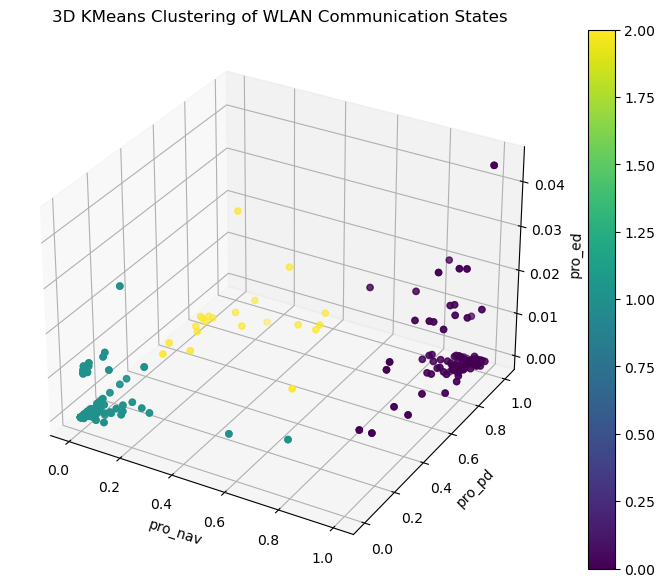
\includegraphics[scale=0.8]{julei2.png}
    \caption{\centering K-eans聚类结果}
    \label{pho:julei2}
\end{figure}

\begin{table}[htp!]
    \centering
    \begin{tabular}{cccc}
        \hline
      & pro\_pd  & pro\_ed  & pro\_nav \\
      \hline
    0 & 0.897140 & 0.003123 & 0.924633 \\
    \hline
    1 & 0.063595 & 0.001679 & 0.034990 \\
    \hline
    2 & 0.770176 & 0.001579 & 0.150017\\
    \hline
    \end{tabular}
    \vspace{0.5cm}
    \caption{聚类所对应门限区间概率}
    \label{tb:julei}
    \end{table}

创建新的特征变量'SINR',根据分类类型,使用5.1.2(2)节提到的计算方法分别计算对应SINR值。

\textbf{(5)数据变换}。对protocol变量,取01变换。筛选并去除RSSI异常值,构造pro\_pd等之前没有筛选,这是为了保证得到的概率值更具真实性,现在使用3σ准则筛选,去除异常值。
随后,为了得到更好的预测效果,对这些数列求平均,得到各RSSI序列的平均强度。

\textbf{(6)主表拆分},观测到训练数据中,每个测试由AP个数行组成,考虑到这些行之间由于在同一个测试场景中,部分RSSI数据具有互补性,将其分割为AP个数个子表,对于AP=2,按照行数对2的余数分为两个子表,对于AP=3,按照行数对3的余数分为3个子表。每个子表对应一个AP在测试中的表现。此时观察到test\_id在子表无意义,移除该变量。

\textbf{(7)相关性分析},接着我们对特征变量: 协议,RSSI, nav,pro\_pd, pro\_ed等进行相关性分析(图\ref{pho:corr})再次剔除了一些具有强线性相关的特征变量。其中
在此基础上,erip 与 ap\_from\_ap\_other\_sum/max/mean\_ant\_rssi 具有强正向线性关系,
将其结合在一起考虑。另外,sta\_to\_ap\_other\_sum/max/mean\_ant\_rssi 和 sta\_from\_ap\_other\_sum/max\_mean\_ant\_rssi 等也汇总在一起考虑,
使用 sum\_rssi 来代表这些 max/mean rssi 指标。
因为我们认为sum值相较于前两者有更多信息,更具有代表性。

\begin{figure}[!htp]
	\centering
	\subfloat[AP0的Pearson相关系数]{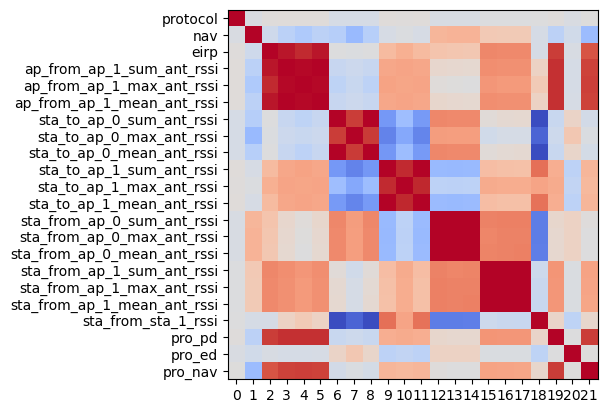
\includegraphics[width=0.4\textwidth]{a0pearson}}\qquad
	\subfloat[AP1的Pearson相关系数]{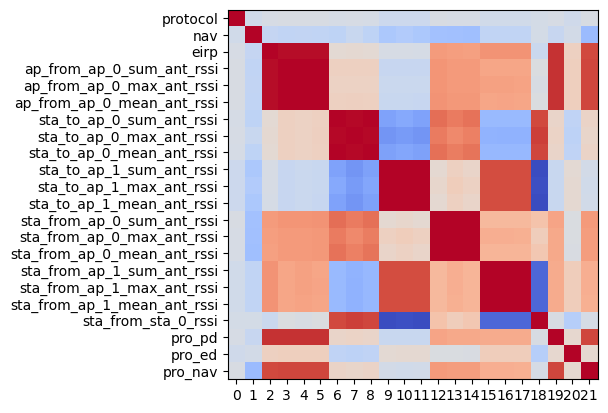
\includegraphics[width=0.4\textwidth]{a1pearson}} \\
	\subfloat[AP0的spearman相关系数]{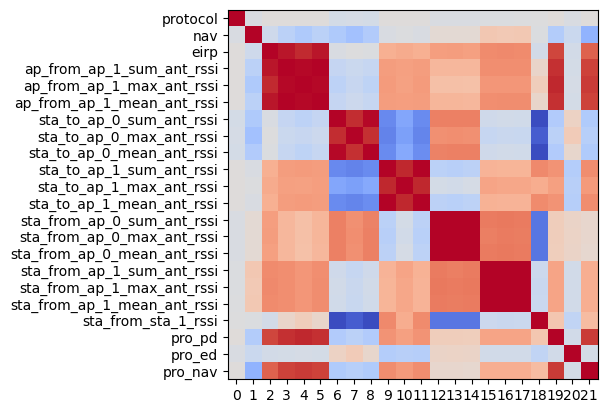
\includegraphics[width=0.4\textwidth]{a0spearman}}\qquad
	\subfloat[AP1的spearman相关系数]{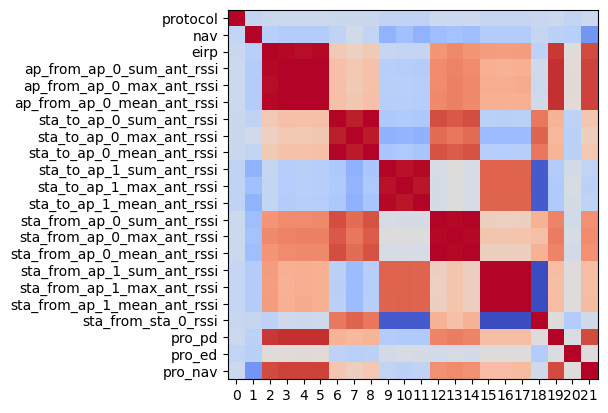
\includegraphics[width=0.4\textwidth]{a1spearman}}
	\caption{AP0和AP1的相关性分析}
    \label{pho:corr}
\end{figure}

\textbf{(8)子表合并},为了提升预测模型输入数据集的大小,我们将AP=2和AP=3的子表分别合并,形成一个新的数据集,以便于后续建模。合并过程中,对主表中互补的特征变量进行对应合并,例如,在AP=2的情境下,AP0的特征ap\_from\_ap\_1\_sum\_ant\_rssi与AP1的特征ap\_from\_ap\_0\_sum\_ant\_rssi合并为ap\_from\_ap\_other\_sum\_ant\_rssi。合并示意如图\ref{pho:hebing},具体合并规则请见附录A。

\begin{figure}[!htbp]
    \centering
    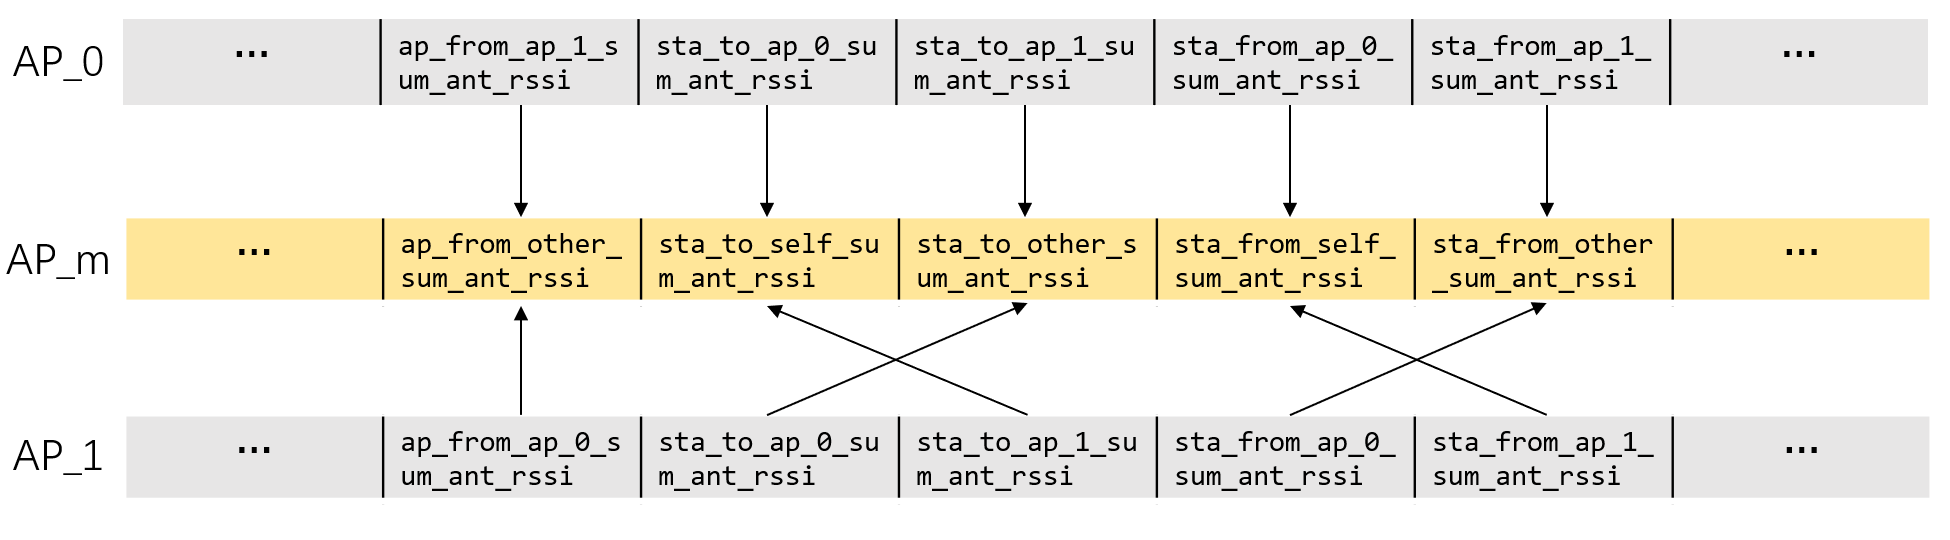
\includegraphics[scale=0.5]{hebing.png}
    \caption{\centering AP子表合并示意图}
    \label{pho:hebing}
\end{figure}
\subsubsection{各参数影响程度排序}
 考虑到目标预测数据seq\_time是连续变量,并且为了充分求解特征变量对目标变量的重要性,我们采用了建模方法:随机森林。

 \textbf{随机森林(Random Forest):}

随机森林是一种集成学习方法,基于决策树构建多个分类或回归模型,然后通过集成多个模型的结果来提高模型的准确性和稳定性。它特别适用于高维数据和非线性数据,具有较强的抗过拟合能力。随机森林的基本思想是通过构建多个决策树,并结合它们的预测结果来做最终决策。其主要特点是通过随机性来减少模型的方差,从而避免过拟合。

随机森林的工作原理是:从原始数据集中随机有放回地抽取多个子集(即 Bootstrap 样本),每个子集大小与原
始数据集相同,但每个样本可能在某个子集中出现多次。对每个子集分别训练一棵决策树。在构建每棵决策树时,随机选取一部分特征进行分裂,避免所有树使用相同的特征进
行建模。这一过程引入了随机性,称为特征随机性。
• 由于每棵树都是在不同的数据子集和特征子集上构建的,所以每棵树都是不同的。对于回归问题,最终的预测值是所有树预测值的平均。

随机森林具有很强的抗拟合性,特别是在数据噪声较多的情况下。观察到本题训练集中变量较多,可推断的具有较强影响的变量较少,结合随机森林的高维数据的处理能力和可解释性,初步使用该模型是个稳健的选择。
 
通过随机森林模型输出的各参数影响程度排序如下:

\begin{figure}[!htbp]
    \centering
    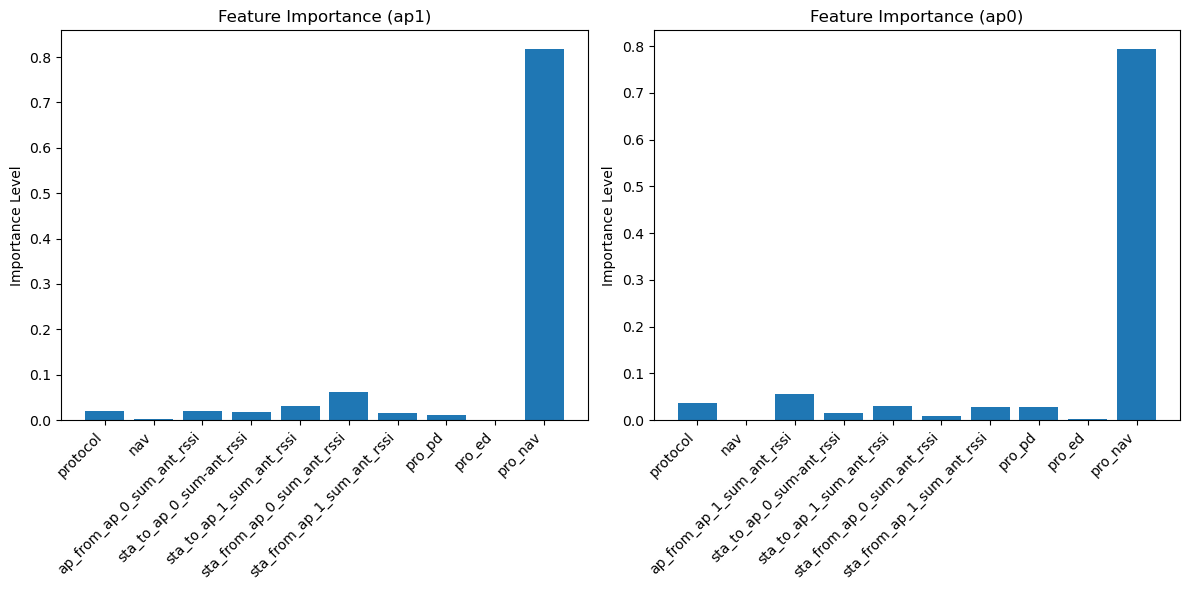
\includegraphics[scale=0.7]{2apinp.png}
    \caption{\centering 2AP情况下各参数影响程度排序}
    \label{pho:2apinp}
\end{figure}

\begin{table}[htp!]
    \centering
    \begin{minipage}{0.45\textwidth}
        \centering
        \begin{tabular}{|c|c|}
            \hline
            \textbf{指标} & \textbf{相关系数} \\
            \hline
            pro\_ed & 0.0204786 \\
            \hline
            nav & 0.00224272 \\
            \hline
            pro\_pd & 0.01946922 \\
            \hline
            sta\_from\_ap\_1\_sum\_ant\_rssi & 0.01885899 \\
            \hline
            sta\_to\_ap\_0\_sum\_ant\_rssi & 0.03116345 \\
            \hline
            ap\_from\_ap\_0\_sum\_ant\_rssi & 0.06179776 \\
            \hline
            protocol & 0.01493922 \\
            \hline
            sta\_to\_ap\_1\_sum\_ant\_rssi & 0.01228365 \\
            \hline
            sta\_from\_ap\_0\_sum\_ant\_rssi & 0.00084504 \\
            \hline
            pro\_nav & 0.81792136 \\
            \hline
        \end{tabular}
        \caption{各特征变量与相关系数 - AP1}
        \label{tab:corresponding_values_ap1}
    \end{minipage}
    \hspace{0.05\textwidth} % 调整两个表格之间的间距
    \begin{minipage}{0.45\textwidth}
        \centering
        \begin{tabular}{|c|c|}
            \hline
            \textbf{指标} & \textbf{相关系数} \\
            \hline
            nav & 0.03613917 \\
            \hline
            pro\_ed & 0.0009684 \\
            \hline
            sta\_from\_ap\_0\_sum\_ant\_rssi & 0.05637722 \\
            \hline
            sta\_to\_ap\_0\_sum\_ant\_rssi & 0.01610746 \\
            \hline
            pro\_pd & 0.02931114 \\
            \hline
            sta\_from\_ap\_1\_sum\_ant\_rssi & 0.0089415 \\
            \hline
            sta\_to\_ap\_1\_sum\_ant\_rssi & 0.02875819 \\
            \hline
            protocol & 0.02802079 \\
            \hline
            ap\_from\_ap\_1\_sum\_ant\_rssi & 0.00144091 \\
            \hline
            pro\_nav & 0.79393525 \\
            \hline
        \end{tabular}
        \caption{各特征变量与相关系数 - AP0}
        \label{tab:corresponding_values_ap0}
    \end{minipage}
\end{table}



我们自己人工根据 $ap\_from\_ap\_other\_mean\_ant\_rssi$ 等指标与 $nav$ 门限所创造的 $pro\_nav$ 最重要,体现了传输方式;其次是 sta\_from\_ap\_other/self\_sum\_ant\_rssi 与 protocol 最重要,最后是 nav 门限与根据 ed 门限和 ap\_from\_ap\_other\_max\_ant\_rssi 等特征,
以及sta\_from\_sta\_0/1等指标。

 \subsubsection{模型建立}
 建立预测模型,我们分别建立了随机森林、XGBoost、Ridge模型进行seq\_time的预测。采用交叉验证法评古模型性能。

 \textbf{XGBoost:}
 对于包含 $n$ 条 $m$ 维的数据集,XGBoost 模型的预测结果可表示为:
 \[
 \hat{y}_i = \sum_{k=1}^{K} f_k(x_i), \quad f_k \in \mathcal{F}, \quad i = 1, 2, \dots, n
 \]
 其中,$\mathcal{F} = \{ f(x) = w_{q(x)} \}$,$q : \mathbb{R}^m \to \{1, 2, \dots, T\}$ 是决策树的结构,表示输入样本被映射到对应叶子节点的路径,$T$ 为叶子节点的数量,$w \in \mathbb{R}^T$ 代表叶节点上的得分值。决策树的结构集合 $\mathcal{F}$ 中的每个函数 $f_k$ 都表示一棵 CART 决策树。
 
 一般来说,损失函数用于衡量模型预测值 $\hat{y}_i$ 与真实值 $y_i$ 之间的差异。对于 $n$ 个样本,采用平方损失函数可表示为:
 \[
 L = \sum_{i=1}^{n} l(y_i, \hat{y}_i^{(t)})
 \]
 
 进一步,目标函数(Objective Function)可以写为:
 \[
 \text{Obj}^{(t)} = \sum_{i=1}^{n} l(y_i, \hat{y}_i^{(t)}) + \Omega(f_t)
 \]
 其中,$\Omega(f_t)$ 表示基模型的复杂度度量,若基模型为决策树,树的深度和叶子节点数等因素都会反映其复杂度。这一正则化项有助于防止模型过拟合。
 
 
 \textbf{岭回归(Ridge Regression):}
 在特征变量的相关性分析中,发现许多变量之间存在显著的线性关系。虽然已进行了一定的特征筛选,但仍可能存在多重共线性问题。为应对这一挑战,拟采用岭回归(Ridge Regression)进行检查与预测。岭回归是一种对线性回归模型的扩展,旨在通过正则化降低因多重共线性导致的过拟合现象。其核心在于向损失函数引入 L2 正则化项,以控制模型复杂度,从而提高泛化能力。

 当特征高度相关时,线性回归的系数可能会变得不稳定,导致模型在训练集上表现优异但在测试集上效果不佳。岭回归通过优化损失函数:
 
 \[
 \text{损失函数} = \sum (y_i - X_i \beta)^2 + \lambda \sum \beta_j^2
 \]
 
 其中,$\lambda$ 为正则化参数,用以调控惩罚项的影响。正则化项 $\sum \beta_j^2$ 旨在限制回归系数的大小,防止模型复杂度过高。
 
 当 $\lambda = 0$ 时,岭回归等价于普通线性回归;随着 $\lambda$ 的增大,回归系数会逐渐缩小,模型复杂度相应降低。
 
 通过这种方式,岭回归有效缓解了多重共线性带来的问题,并提升了模型在新数据上的表现。
 
 \subsubsection{结果对比}
 对于模型预测结果,采用 K 折交叉验证 (k-fold cross-validation) 的方法将数据集划分
 成 K 等分,依次取每一份作为测试集,剩下的 K − 1 份为训练集。交叉验证重复 K 次,
 取 K 次准确率的平均值作为最终模型的评价指标。在我们的验证中,K值取10,分别对三个模型的预测
 结果进行了评估。结果如表\ref{tb:compare1}所示。

 \begin{table}[htp!]
    \centering
    
    \begin{tabular}{ccc}
      \hline %\toprule
      模型    &   最高R*2系数   &  交叉验证 \\
      \hline %\midrule      
      %\rowcolor[gray]{0.90}
      随机森林       &   0.96   &  0.87\\
      \hline
      XGBoost       &    0.94 &  0.87\\
      \hline
      岭回归      &    0.94 &   0.87\\
      \hline
    \end{tabular}
    \vspace{0.5cm}
    \caption{三种模型准确率对比}
      \label{tb:compare1}
    \end{table}
 由表上表数据对比可知,随机森林模型的准确率最高,因此我们选择随机森林模型对test表进行预测。根据题目要求对测试集test\_set\_1\_2ap和test\_set\_1\_3ap中AP发送数据帧序列的总时长进行预测,并填写在对应数据位中。
 
\newpage
\section{问题二的分析与求解}
\subsection{问题分析}
\subsubsection{问题简述}
问题二主要研究AP在发送过程中选用的调制编码方案(Modulation and Coding Scheme, MCS)和空间流数(Number of Spatial Stream, NSS)表征。题目中要求,通过分析实测训练集中的测试基本信息,特别是节点间RSSI信息和门限信息进行分析,针对测试中AP发
送数据选用最多次数的(MCS, NSS)\cite{rn5}进行建模,使用得到的预测模型预测test\_set\_2\_2ap和test\_set\_2\_3ap中的(MCS, NSS)。

\textbf{“选用最多次数的(MCS, NSS)”}理解:经观察,训练集中每一行测试数据都给定了一组(MCS, NSS),我们认为这是AMC算法在测试初始阶段快速收敛后所得到的,并在余下的大部分测试期间都使用这一组(MCS, NSS)用于解调信号,即选用最多次数的(MCS, NSS)。

通过得到这一数值对(MCS, NSS),可以一定程度上表示AP发送数据的PHY层速率(PHY Rate),其可以作为求解第三问系统吞吐量的前置影响条件。

\subsubsection{机制分析}
在WLAN网络中,AP的调制编码方案(MCS)和空间流数(NSS)是影响物理层速率的重要因素。MCS表示调制方式和编码速率的组合,NSS表示数据可以通过多少空间流同时传输。这两个参数会影响AP的PHY层速率(PHY Rate),从而影响数据传输的效率。

通常情况下,AP根据信道条件(如RSSI和信干噪比(SINR))以及网络环境动态调整MCS和NSS。其调节过程通过自适应调制编码(AMC)算法完成。在较好的信道条件下,AMC算法会选择高阶调制方案和较高的NSS,以提高传输速率;而在信道条件较差时,AMC算法会选择低阶调制和较低的NSS,以保证传输的可靠性。

因此,预测AP的MCS和NSS实际上是通过了解信道质量以及AP的传输环境,模拟AMC算法的决策过程。这一过程受RSSI、SINR、CCA门限、NAV机制等影响。
\subsubsection{求解思路}
针对上述问题,提出如下求解思路:

由题目可知,AP发送数据时的PHY层速率PHY Rate取决于调制编码方案MCS和空间流数NSS,而这两者(MCS, NSS)又由信号解调时的SINR决定。WLAN采用AMC自适应调制解调算法,平衡当前SINR下所支持的(MCS, NSS)数值大小,以保证丢包率不高于一定阈值。因此,处理本题时,需要通过测试信息,初步计算信道SINR信息,以进一步预测对应的(MCS, NSS)。

AP的AMC所选用的(MCS, NSS)不仅与SINR相关,同时也与AP的传输方式相关。可以总结的,两个AP之间的传输方式有三种可能:同步传输、异步传输、同步异步混合传输。在各个传输方式下,因为STA接收数据时受到的干扰来源不同,导致SINR的计算方法也不同。因此,为了计算信道SINR信息,需要确定各测试数据所处的传输方式,而这一过程需结合问题一中使用节点间RSSI信息和门限信息进行分类的方法。

为解决问题二,我们首先根据节点间RSSI信息和门限信息对其所处\textbf{传输方式}进行分类,随后根据其实际传输方式用不同的计算方式得到对应\textbf{SINR信息},进一步地,利用SINR对\textbf{(MCS, NSS)}数值进行预测。
本题的数据处理过程仍然沿用第一题的方法,但是去除了主表拆分和合并的过程,这是因为我们发现分表后,子表之间的特征分析具有很大相似性,故直接使用全部数据进行分析。

在预测过程中,我们发现,尽管预测得到的MCS值具有很大的波动性,但是NSS值相对稳定,维持在NSS2附近。这一表现难以评价模型的准确性和拟合效果,因此,我们改为预测MCS和PHY Rate值,
评价模型预测效果,随后利用文中提到的(MCS, NSS)与PHY Rate对应关系,得到对应的NSS,填写预测结果。

问题二思路如图\ref{pho:wenti2}:
\begin{figure}[!htbp]
    \centering
    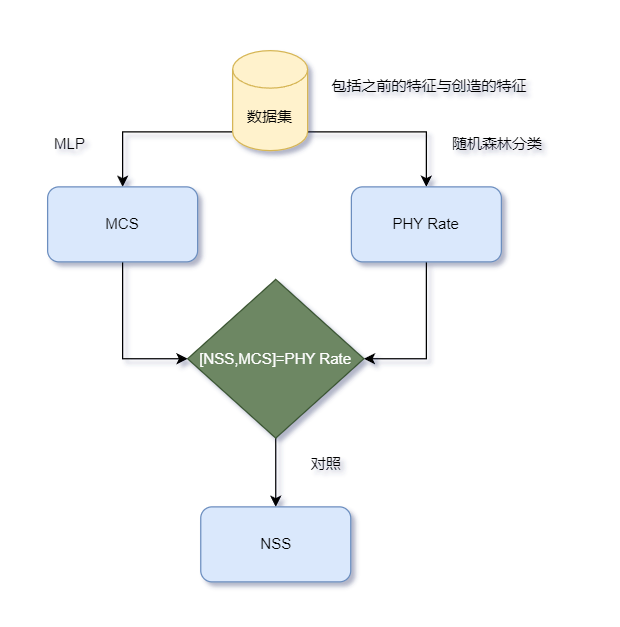
\includegraphics[scale=0.7]{wenti2.png}
    \caption{\centering 问题二思路示意图}
    \label{pho:wenti2}
\end{figure}

\subsection{问题求解}
\subsubsection{数据处理}
在第一问处理的基础上,本问题进一步确定了因为AP间RSSI所处门限区间,用以分类其在一次测试中的主要传输方式,以此进一步计算SINR数值。

\subsubsection{模型构建}
由题目得知,无线信道具有瞬息万变的特点,实测中所测量的RSSI信息属于大尺度信息,不足以完全反应真实信道变化,因此,我们使用
多层感知机(MLP, Multilayer Perceptron)辅助进行目标值预测。

\textbf{多层感知机(MLP, Multilayer Perceptron)}:MLP是一种经典的前馈神经网络,由输入层、一个或多个隐藏层以及输出层构成。MLP 是一种全连接网络,即每一层中的每个神经元都与下一层的所有神经元相连,主要用于处理结构化数据以及分类和回归任务。

\begin{itemize}
    \item 输入层操作:我们对数据进行标准化操作,输入数据的维度决定了输入层神经元的数量,此外输入层不进行任何其他计算,功能是将输入数据传递给下一层。
    \item 隐藏层操作:隐藏层在 MLP 中担任核心角色,其中包含了多个神经元,并通过线性变换与非线性激活函数对输入数据进行处理。隐藏层与上一层所有神经元紧密相连,并从输入数据中提取复杂的模式和特征。该模型中前向传播用于将输入数据通过每一层神经网络,最终产生输出。反向传播则通过计算输出与真实标签的误差(损失函数)来更新权重和偏置,常用的优化算法是梯度下降和 Adam。在此我们使用了两层隐藏层,以充分探索数据集中的复杂关系,并使用 Adam 优化器来对模型进行训练。
    \item 激活函数:
    \begin{itemize}
        \item ReLU(Rectified Linear Unit):常用于隐藏层,ReLU 函数定义为 
        \[
        f(x) = \max(0, x)
        \]
        它能够引入非线性,同时避免梯度消失问题。
        \item Sigmoid:适用于概率预测,输出值在 $(0, 1)$ 之间。
        \item Tanh:将输入压缩到 $(-1, 1)$ 范围,常用于对数据中心化的任务。
    \end{itemize}
    在该模型中,我们使用了 ReLU 激活函数,因为最后预测结果并不需要对输出范围进行限制。
    \item 前向传播与反向传播: MLP 的训练过程基于前向传播和反向传播。
    \item 正则化技术:为防止过拟合,MLP 中常采用正则化技术,例如 Dropout 和 L2 正则化。Dropout 随机丢弃一部分神经元的连接,减少模型对特定权重的依赖,提高模型的泛化能力。在模型中我们针对隐藏层的输出结果进行了 $0.2$ 概率的 Dropout。
\end{itemize}

\subsubsection{结果分析}

\begin{figure}[!htbp]
    \centering
    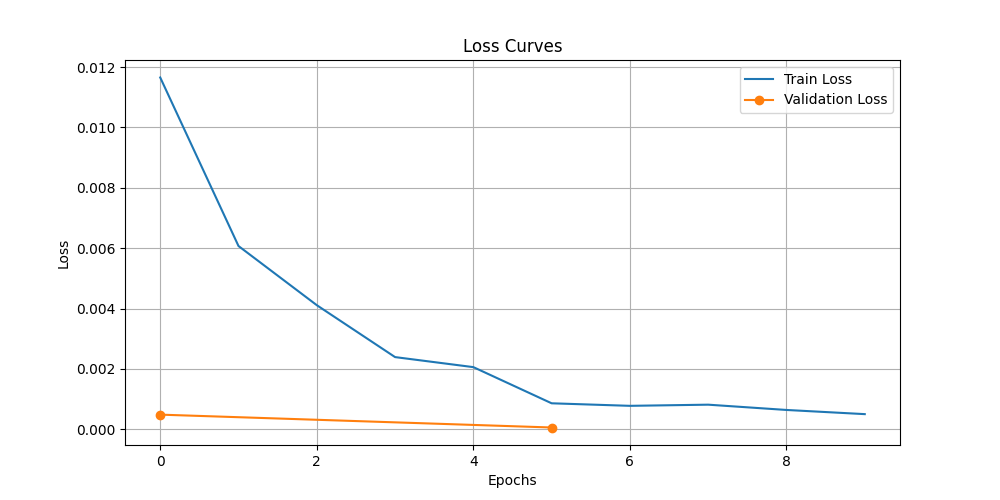
\includegraphics[scale=0.7]{mlploss.png}
    \caption{\centering MLP模型训练过程}
    \label{pho:mlploss}
\end{figure}

由上图可知,模型在训练集和验证集上的损失值逐渐下降,且在验证集上的损失值与训练集上的损失值保持一致,说明模型具有较好的泛化能力。但是因为用于训练的数据集很小,所以仅训练了较少的epoch。

\textbf{同频AP个数为2:}

使用10折交叉验证对预测结果的PHY Rate进行评估,得到的R2系数均值为0.89,10次测验的值分别为:[0.91014529, 0.97066302, 0.83193871, 0.95018807, 0.96852579,
0.75103629, 0.94168775, 0.80378873, 0.95456839, 0.83780847]。

使用10折交叉验证对预测结果的MCS进行评估,得到的R2系数均值为0.91,10次测验的值分别为:
[0.84210526, 0.92105263, 0.89473684, 0.92105263, 0.89473684,0.92105263, 0.86842105, 0.94736842, 0.92105263, 0.97297297]。

\textbf{同频AP个数为3:}

使用10折交叉验证对预测结果的PHY Rate进行评估,得到的R2系数均值为0.85,10次测验的值分别为:[0.91701557, 0.86328318, 0.87501772, 0.86086456, 0.84691466,
0.80411334, 0.82224948, 0.84631725, 0.84689186, 0.88545755]

使用10折交叉验证对预测结果的PHY Rate进行评估,得到的R2系数均值为0.86,10次测验的值分别为:[0.91701557, 0.86328318, 0.87501772, 0.86086456, 0.84691466,
       0.80411334, 0.82224948, 0.84631725, 0.84689186, 0.88545755]

上述结果证明模型预测较为准确,且通过观察10次结果可知,模型具有较好的鲁棒性。

如6.1.3节末尾处提到,此处没有评估和预测NSS值,因为预测结果的MCS值具有很大的波动性,但是NSS值相对稳定,维持在NSS2附近。这一表现难以评价模型的准确性和拟合效果,因此,我们改为预测NSS和PHY Rate值,评价模型预测效果,随后利用文中提到的(MCS, NSS)与PHY Rate对应关系,得到对应的MCS,填写预测结果。
\newpage
\section{问题三的分析与求解}
\subsection{问题分析}
\subsubsection{问题简述}
问题三主要研究WLAN网络系统吞吐量预测。题目要求结合问题一和问题二的分析,利用前两问的预测指标,包括AP发送数据帧序列的总时长、(MCS, NSS)以及其他测试基本信息,共同构建预测模型,通过测试集test\_set\_1\_2ap和test\_set\_1\_3ap预测网络吞吐量。其中问题二所预测得到的(MCS, NSS)无法获得很高精度,允许采用实测中统计的数据帧真实(MCS, NSS)作为模型输入变量。

问题三是本课题的最终研究目标,前两问通过分析WLAN网络拓扑、节点间RSSI、信道接入机制、干扰等因素对WLAN数据发送、速率的影响,本问题进一步地利用其预测结果作为重要影响因素与支撑,对WLAN系统吞吐量进行精确预测。基于该吞吐量预测模型,对WLAN进行优化,有望突破工业、教育、医疗等新场景,为用户提供极致的业务体验。


\subsubsection{机制分析}

根据题目背景,给出如下定义:
\begin{itemize}
    \item 吞吐量(throughput):吞吐量指节点单位时间内成功发送的比特数。仅MSDU的总字节数是有效传输数据,进行吞吐量计算。
    \item 丢包率(per):发送数据帧的失败个数与总个数的百分比。
    \item 数据的帧序列的总时长(seq\_time)(us):所有成功或失败的数据帧发送,帧序列时长从开始发送RTS到收到ACK,或者超时。
    \item 数据帧的时长($T_{\text{PPDU}}$) (s):一个数据帧的时长。一次测试里,统计每个数据帧的时长,取平均值。仅包括PPDU的传输时间,不包括RTS,ACK等。
    \item AMPDU个数($N_{\text{AMPDU}}$):一个数据帧的聚合个数。一次测试里,统计每个数据帧的聚合个数,取平均值。聚合的详细解释见第4节。
    \item TCP的ACK算是数据帧,算作吞吐量,个数是下行数据帧的3:1到2:1左右。根据丢包率改变传输速率。ACK的大小为64Bytes。
    UDP仅计算AP发往STA的数据帧,发送时间间隔服从泊松分布,发送数据的速率为290 Mbps。
\end{itemize}

\textbf{(1)数据包长度分析:}

设$N_{\text{success}}$为一次时长60s的测试中成功发出的数据包的个数。$N_{\text{timeout}}$为测试中失败的包的个数,有:
\begin{align}
    T_{\text{seq\_time}} = N_{\text{timeout}} \times T_{\text{timeout}} + N_{\text{success}} \times T_{\text{success}} \label{eq:seq_time}
    \end{align}

其中,$T_{\text{success}}$为成功发送数据帧的时长,即$T_{\text{PPDU}}$;$T_{\text{timeout}}$为失败发送数据帧的时长,根据\ref{pho:rtscts2}可知,传输失败时时长包括RTS时长与超时时长,即$T_{\text{timeout}} = T_{\text{RTS}} + T_{\text{ACK\_timeout}} = 85 \, \mu s$。

\begin{figure}[!htbp]
    \centering
    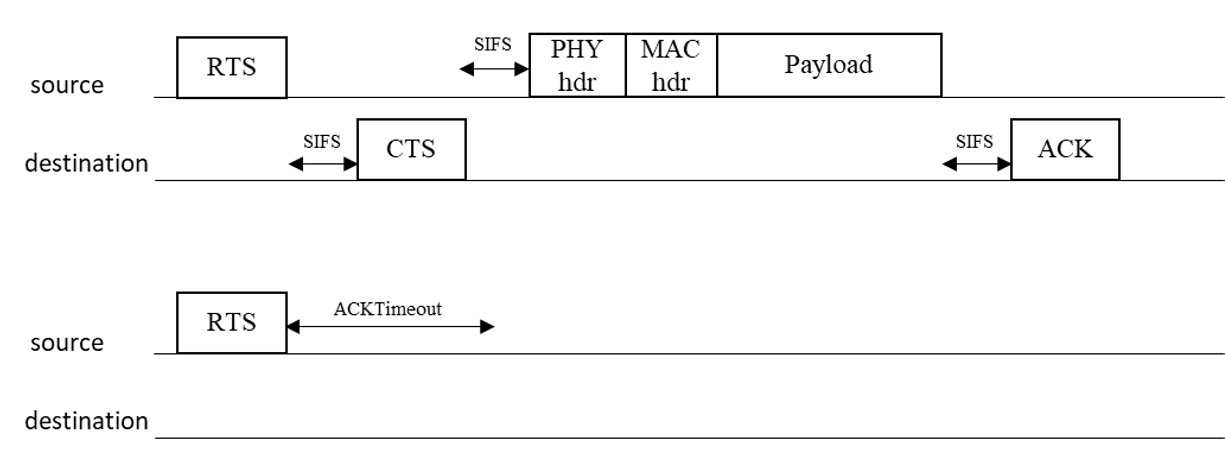
\includegraphics[scale=0.8]{rtscts2.png}
    \caption{\centering RTS-CTS模式下发送成功发送失败的帧序列}
    \label{pho:rtscts2}
\end{figure}

又由丢包率定义可知,$\text{PER} = \frac{N_{\text{timeout}}}{N_{\text{success}}+N_{\text{timeout}}}$,变换得:
\begin{align}
    N_{\text{timeout}} = \frac{\text{PER}}{1-\text{PER}} \times N_{\text{success}} \label{eq:y}
    \end{align}

因此,由式\ref{eq:seq_time}与式\ref{eq:y}可得:
% \begin{align}
%     T_{\text{seq\_time}} = \frac{\text{PER}}{1-\text{PER}} \times N_{\text{success}} \times T_{\text{timeout}} + N_{\text{success}} \times T_{\text{success}}\label{eq:seq_time2}  
%     \end{align}
\begin{align}
    N_{\text{success}} = \frac{T_{\text{seq\_time}}}{T_{\text{success}} + \frac{\text{PER}}{1-\text{PER}} \times T_{\text{timeout}}}  \label{eq:x}
    \end{align}

    记测试中一个PPDU数据包的长度为$L_{\text{PPDU}}$对于吞吐量$\text{Throughput}$(MBps),有,
\begin{align}
    \text{Throughput} = \frac{N_{\text{success}} \times L_{\text{PPDU}} \times 8.0}{60 \times 10^6} \label{eq:throughput}
    \end{align}

即,
\begin{align}
    L_{\text{PPDU}} = \frac{\text{Throughput} \times 60 \times 10^6}{N_{\text{success}} \times 8} \label{eq:throughput}
    \end{align}

    综上所述,在训练集中,吞吐量已给出的情况下,我们可以利用吞吐量、丢包率和数据帧发送总时长,计算出测试中聚合数据包PPDU的平均长度。

\textbf{(2)聚合参数分析:}

为了提升发送小包的效率,协议允许通过聚合一次发送多个具有相同目的地址的数据包\cite{rn4},如\ref{pho:juhe2}。在一次数据包聚合(AMSDU)过程中,多个相同接收地址的同服务类别的MAC服务数据单元(MSDU)封装成一个MAC协议数据单元(MPDU)。组装好的多个MPDU进一步聚合(AMPDU),这一过程包括将多个MPDU聚合成一个PHY协议数据单元(PPDU)。此处PPDU即为在WLAN网络中进行传输的一个数据帧。
\begin{figure}[!htbp]
    \centering
    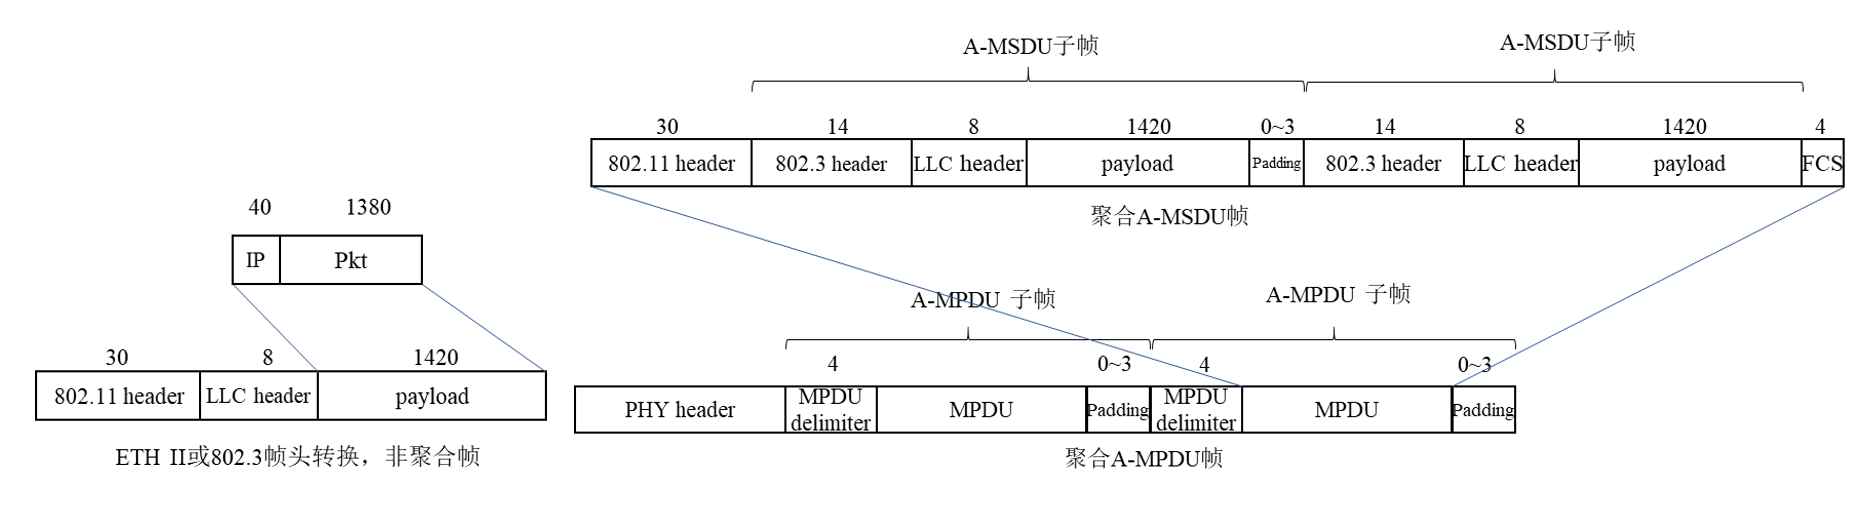
\includegraphics[scale=0.5]{juhe.png}
    \caption{\centering 聚合数据包示意图}
    \label{pho:juhe2}
\end{figure}

组成MPDU的MSDU包长计算如式\ref{eq:msdu}(单位:Bytes):
\begin{align}
    L_{\text{MSDU}} = L_{\text{802.3header}} + L_{\text{LLCheader}} + L_{\text{payload}} + L_{\text{padding}} \label{eq:msdu}
    \end{align}

其中,802.3header为14Bytes,LLCheader为8Bytes,此处payload即为测试基本信息中的'pkg\_len',长度为1500Bytes。AMSDU过程中需插入0-3字节的填充字节进行4字节对齐,此处padding计算可得为2Bytes。   

组成PPDU的MPDU包长计算如式\ref{eq:mpdu}(单位:Bytes):
\begin{align}
    L_{\text{MPDU}} = L_{\text{802.11header}} + L_{\text{MSDU}} \times N_{\text{AMSDU}} - L_{\text{padding}} + L_{\text{FCS}} \label{eq:mpdu}
        %  &= 30 + 1524 \times num\_AMSDU - 2 + 4 \label{eq:mpdu}\\
        %  &= 32 + 1524 \times num\_AMSDU \nonumber
    \end{align}

其中,802.11header为30Bytes,FCS为4Bytes。

最终,计算一个完整数据帧PPDU的包长(单位:Bytes)式\ref{eq:ppdu}:
\begin{align}
    L_{\text{PPDU}} = (L_{\text{delimiter}} + L_{\text{MPDU}} + L_{\text{padding}}) \times N_{\text{AMPDU}} + L_{\text{PHY}} \label{eq:ppdu}
\end{align}


其中,$L_{\text{delimiter}}$为4Bytes,PHY为PHY头部大小。在802.11 WLAN中\cite{rn2,rn3},最常见的PHY头部大小通常是160位(20字节),适用于802.11a、802.11g、802.11n、802.11ac和802.11ax等标准。这是因为这些标准大多数都基于OFDM(正交频分复用)调制,采用相同的PHY头部结构对于802.11b(DSSS和CCK),虽然它的PHY头部是192位(24字节),但在现代无线网络中,802.11a/g/n/ac/ax的使用更为广泛,因此160位的PHY头部是最常见的。此外,不同的PHY头字节数差异不大,我们认为对最终结果的造成误差可以忽略不计。

已知PPDU长度(即$L_{\text{PPDU}}$),且
\begin{align}
    L_{\text{padding}} =4 - L_{\text{MPDU}} \% 4 \label{eq:padding}
    \end{align}

则$L_{\text{MPDU}}$可以根据如下计算得出,联立\ref{eq:padding}与\ref{eq:ppdu},带入已知数值:
\begin{align}
    L_{\text{MPDU}} - L_{\text{MPDU}}\%4 = \frac{L_{\text{PPDU}} - 20}{N_{\text{AMPDU}}} - 8 \label{eq:mpdu2}
    \end{align}
    
由$L_{\text{MPDU}}\%4 \in [0,3]$,可以认为
\begin{align}
    L_{\text{MPDU}} = \frac{L_{\text{PPDU}} - 20}{N_{\text{AMPDU}}} - 8 + r, \quad r \in [0,3] \label{eq:mpdu3}
    \end{align}
    
    由于MPDU实际值很大(几千bytes),则不妨取r=0,又因为一个MSDU的长度为1524bytes(式\ref{eq:msdu}),可得:
    \begin{align}
        L_{\text{MPDU}} = 32 + 1524 \times N_{\text{AMSDU}} \label{eq:mpdu4}
        \end{align}

联立\ref{eq:mpdu3}和\ref{eq:mpdu4}两式可得:
\begin{align}
    N_{\text{AMSDU}} = \frac{\left(\frac{L_{\text{PPDU}} - 20}{N_{\text{AMPDU}}} - 40\right)}{1524} \label{eq:amnsu}
    \end{align}

综上,在已知$L_{\text{PPDU}}$的情况下,我们可以得到$N_{\text{AMSDU}}$和$N_{\text{AMPDU}}$之间的关系表达式,由于训练集中没有
给出AMSDU聚合包个数$N_{\text{AMSDU}}$的对应值,我们可以通过训练集中给定的吞吐量等数据,通过式\ref{eq:throughput}计算出聚合数据包 PPDU 的平均长度$L_{\text{PPDU}}$,随后利用
同样给出的AMPDU聚合包个数$N_{\text{AMPDU}}$,通过式\ref{eq:amnsu}计算出AMSDU聚合包个数。

\subsubsection{求解思路}

根据题目可知,WLAN网络吞吐量主要取决于AP发送机会、发送时所选用的PHY Rate以及数据帧的比特数。其中,AP发送机会即为问题一中的seq\_time,PHY Rate可以根据下表映射到问题二中所预测的(MCS, NSS)。本问题中,
主要通过分析数据帧比特数对吞吐量的影响。

吞吐量指节点单位时间内成功发送的比特数,而有效传输数据仅包括 MSDU 的总字节数。因此,我们认为,深度挖掘聚包机制是具有意义的,其中使用的参数在预测系统吞吐量
过程中,具有较高参考价值,其中,数据帧的时长$T_{\text{PPDU}}$、AMSDU聚合个数$N_{\text{AMSDU}}$和AMPDU聚合个数$N_{\text{AMPDU}}$参数被认为具有代表性。
然而通过观察测试集发现,上述几个变量均未给出。因此我们希望先通过类似一、二两问的预测过程,先得出$T_{\text{PPDU}}$、$N_{\text{AMSDU}}$和$N_{\text{AMPDU}}$的预测值,并用于
新的模型输入,用来预测吞吐量。

问题三思路如图\ref{pho:wenti3}:
\begin{figure}[!htbp]
    \centering
    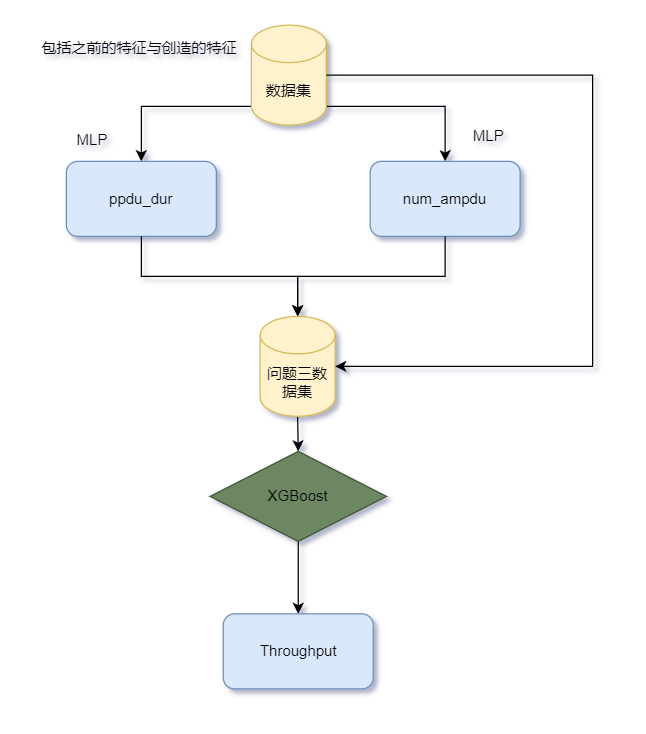
\includegraphics[scale=0.7]{wenti3.png}
    \caption{\centering 问题三思路示意图}
    \label{pho:wenti3}
\end{figure}

\subsection{问题求解}

\subsubsection{模型构建}

本问题中,先用多层感知机MLP模型预测出$T_{\text{PPDU}}$和$N_{\text{AMPDU}}$作为预测值,随后,使用XGBoost模型预测得到吞吐量。
此处,根据散点图\ref{pho:3pearson}可知,$N_{\text{AMSDU}}$与$N_{\text{AMPDU}}$呈现正相关,系数为0.6,且相关性较高,故只考虑$T_{\text{PPDU}}$和$N_{\text{AMPDU}}$作为特征变量。

\begin{figure}[!htbp]
    \centering
    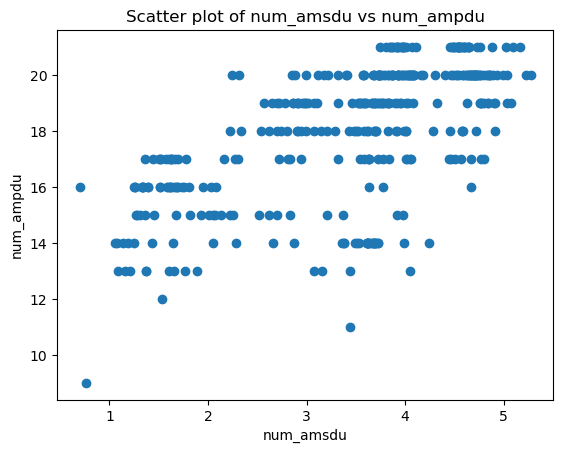
\includegraphics[scale=0.7]{3pearson.png}
    \caption{\centering $N_{\text{AMSDU}}$与$N_{\text{AMPDU}}$关系展示图}
    \label{pho:3pearson}
\end{figure}

\subsubsection{结果分析}

问题3中ap2对于throughoutput的值回归,均值为0.96,10折验证结果为array([0.97346603, 0.96983368, 0.97503999, 0.93833553, 0.93052316,
       0.98189316, 0.97710122, 0.96557072, 0.94913004, 0.95445993])

问题3中对于ap3对于throughoutput的值的回归,均值为0.95,10折交叉验证结果为array([0.97497345, 0.98397   , 0.95935381, 0.97253042, 0.97065528,
0.95160585, 0.97799428, 0.95418978, 0.96758076, 0.9685466 ])

由结果可知,模型预测效果良好,且鲁棒性较强。

\newpage
\section{模型总结}

\subsection{方案优点}

本文在充分WLAN机制的基础上,对数据集进行了特征创造,用概率的方式体现同频AP之间通信的模式。该人工特征在后续的特征重要程度排名中名列前茅,证明了该人工特征的合理性与有效性。

本文从一开始解决问题的时候,就利用最大条件引入了后续可能用到的特征,如SINR,聚类状态等信息,并采用多个模型和算法进行分析,最大程度上利用数据集中的信息。

本文对于所有题目中2AP与3AP的情况进行了分开讨论,针对容易模拟的2AP情形,对使用的模型进行横向对比,至于情况复杂多变的3AP情形,使用多层感知机来探究其复杂关系。

在针对包聚合问题的时候,采用机理分析与深度学习预测相结合的方式,填补了其中所需要的缺失参数,并成功对目标值进行预测。

\subsection{方案不足}

用来给深度学习模型训练的数据集的数量并不是很多,深度学习模型预测的参数效果可能会差强人意,同时基于预测值所分析的结果质量也会下降;

模型如MLP,XGBoost等模型预测性能虽然很好,但是解释性相对较差,若要在相关领域进行预测分析,可能需要改进并更新对应的模型解释工具。

\subsection{未来的改进方向}

获得更多的真实数据,并将基站的位置信息等多方面特征因素纳入考虑,提高模型的鲁棒性和稳定性;

可以考虑模型融合技术或启发式算法优化模型技术,将多个模型的预测结果进行融合,或者对模型效果进行优化。

\bibliographystyle{gmcm}
\bibliography{reference}






\section{附录A 题目测试集结果}
% \documentclass{article}


\begin{longtable}{ll}
\caption{test\_set\_1\_2\_ap} \\ % 表格标题
\hline
\textbf{Predict Seq Time} & \textbf{Predict Throughput} \\ 
\hline
\endfirsthead

\hline
\textbf{Predict Seq Time} & \textbf{Predict Throughput} \\ 
\hline
\endhead

\hline
\endfoot

47.2651           & 124.665            \\
48.3345           & 133.4773           \\
49.8563           & 141.9504           \\
50.1373           & 156.6426           \\
47.2461           & 129.1914           \\
48.5465           & 139.6945           \\
49.1479           & 141.9945           \\
50.2585           & 159.6448           \\
47.2017           & 129.3225           \\
48.0187           & 137.0568           \\
49.0428           & 144.9029           \\
50.4356           & 156.3343           \\
47.7852           & 128.562            \\
48.1161           & 147.953            \\
49.6241           & 140.187            \\
50.2939           & 146.1679           \\
47.3202           & 150.0952           \\
48.1482           & 128.1342           \\
49.2009           & 163.1809           \\
50.336            & 165.8982           \\
47.8155           & 145.9913           \\
48.1552           & 146.455            \\
49.4027           & 165.9966           \\
50.3686           & 141.2401           \\
47.7371           & 146.6508           \\
48.3117           & 169.0632           \\
49.0145           & 180.0328           \\
50.2669           & 184.9271           \\
47.1948           & 150.6723           \\
47.9691           & 154.1246           \\
49.3971           & 177.8843           \\
50.0384           & 179.9314           \\
46.2543           & 164.0636           \\
48.2259           & 158.411            \\
48.7257           & 182.3656           \\
50.2888           & 192.1225           \\
41.9092           & 150.6678           \\
48.2105           & 173.6938           \\
44.7022           & 158.3659           \\
49.9435           & 186.3889           \\
34.9224           & 131.2143           \\
46.7297           & 154.9227           \\
36.7786           & 137.9985           \\
49.1878           & 175.1451           \\
35.1717           & 129.7112           \\
44.3223           & 160.4146           \\
38.1973           & 147.8302           \\
48.3467           & 132.1562           \\
34.1428           & 143.9704           \\
40.2908           & 84.4042            \\
36.131            & 150.7141           \\
45.1864           & 106.31             \\
28.8219           & 136.6747           \\
40.0162           & 83.4793            \\
30.1281           & 147.7851           \\
45.2789           & 96.9388            \\
29.5895           & 134.8225           \\
31.762            & 95.4797            \\
32.806            & 153.1011           \\
33.0985           & 98.1278            \\
28.9542           & 139.0358           \\
24.2376           & 83.0778            \\
30.9204           & 148.2933           \\
27.1482           & 88.6441            \\
33.8094           & 145.8498           \\
23.6982           & 85.8838            \\
29.3689           & 141.2124           \\
23.5351           & 84.7705            \\
31.3739           & 152.7492           \\
26.2432           & 88.7686            \\
28.3373           & 138.2543           \\
24.1125           & 88.368             \\
29.8817           & 151.4965           \\
25.409            & 92.314             \\
27.6467           & 129.4512           \\
23.6852           & 75.2333            \\
26.9599           & 134.9168           \\
23.414            & 86.954             \\
29.6329           & 145.4149           \\
24.6413           & 91.1731            \\ 
\end{longtable}



\begin{longtable}{ll}
\caption{test\_set\_1\_3\_ap} \\ % 表格标题
\hline
\textbf{Predict Seq Time} & \textbf{Predict Throughput} \\ 
\hline
\endfirsthead

\hline
\textbf{Predict Seq Time} & \textbf{Predict Throughput} \\ 
\hline
\endhead

\hline
\endfoot

25.0064           & 23.3511            \\
37.4308           & 38.4647            \\
41.4869           & 52.7878            \\
32.53             & 33.9107            \\
36.4835           & 37.5621            \\
37.2803           & 35.3279            \\
24.0461           & 25.4492            \\
42.0029           & 53.5889            \\
41.0497           & 52.4553            \\
21.903            & 26.9922            \\
42.2178           & 52.8659            \\
41.6774           & 50.0746            \\
30.7003           & 38.0648            \\
39.532            & 49.4355            \\
35.5419           & 34.2947            \\
23.7177           & 26.3978            \\
39.2109           & 47.8945            \\
41.405            & 54.3591            \\
22.7145           & 48.5024            \\
44.1882           & 59.132             \\
41.9338           & 50.4032            \\
25.5747           & 55.6519            \\
44.0885           & 67.5784            \\
37.0978           & 34.2534            \\
20.2587           & 42.5505            \\
39.7868           & 58.9801            \\
38.9722           & 91.9616            \\
24.652            & 54.5131            \\
36.9085           & 70.756             \\
33.0503           & 82.0039            \\
23.6014           & 68.1198            \\
41.4522           & 58.5663            \\
25.1013           & 87.1511            \\
24.837            & 70.3053            \\
40.4583           & 65.1086            \\
29.3328           & 54.14              \\
23.3822           & 67.4068            \\
36.5983           & 56.4485            \\
26.6571           & 86.1911            \\
25.8175           & 57.8042            \\
33.6015           & 49.6523            \\
30.3998           & 84.6175            \\
25.0081           & 58.6933            \\
36.601            & 39.9178            \\
24.1975           & 67.3314            \\
26.5525           & 73.7755            \\
33.0559           & 49.8761            \\
22.2881           & 58.4201            \\
26.8027           & 57.1233            \\
32.6059           & 55.6853            \\
30.2375           & 81.7713            \\
27.205            & 77.3873            \\
29.9736           & 47.8943            \\
23.3535           & 69.7504            \\
27.6127           & 61.2838            \\
30.8926           & 47.7008            \\
24.8584           & 68.4584            \\
22.7993           & 48.1896            \\
32.0543           & 87.9842            \\
22.437            & 60.3641            \\
22.41             & 48.6827            \\
25.8643           & 50.0561            \\
23.8022           & 75.7764            \\
22.1196           & 60.714             \\
25.4878           & 67.5494            \\
21.0649           & 68.869             \\
22.1639           & 61.8667            \\
23.5779           & 67.1891            \\
22.5061           & 66.8044            \\
23.6727           & 55.5947            \\
26.5288           & 60.5337            \\
23.9582           & 64.0304            \\
21.7973           & 61.7426            \\
23.7318           & 66.992             \\
22.7815           & 66.1026            \\
21.9857           & 63.9706            \\
24.208            & 67.7197            \\
22.8256           & 68.0849            \\
22.5585           & 43.1276            \\
26.0471           & 62.9898            \\
24.9793           & 64.1981            \\
20.1463           & 60.1995            \\
23.4939           & 68.5515            \\
23.0938           & 67.8585            \\
22.3694           & 42.795             \\
26.1427           & 39.0985            \\
23.3986           & 66.8948            \\
20.6397           & 62.1902            \\
23.3422           & 67.9997            \\
22.7726           & 67.2747            \\
22.6451           & 44.8699            \\
24.8425           & 58.0489            \\
24.4456           & 70.1642            \\
21.524            & 63.8814            \\
23.8503           & 70.0541            \\
22.6385           & 67.6238            \\
22.5524           & 49.043             \\
26.1925           & 60.826             \\
23.8125           & 62.6679            \\
21.2791           & 61.8713            \\
23.116            & 67.2642            \\
22.1655           & 66.8284            \\
21.372            & 40.4767            \\ 
25.1866           & 39.7041            \\
23.6661           & 69.6283            \\ 
\end{longtable}



\begin{longtable}{llll}
\caption{test\_set\_2\_2\_ap} \\ % 替换为表格标题
\hline
seq\_time & predict nss & predict mcs & PHY\_rate \\
\hline
\endfirsthead
\hline
seq\_time & predict nss & predict mcs & PHY\_rate \\
\hline
\endhead
\hline
\endfoot
\hline
\endlastfoot
48.399    & 2           & 5           & 117.648   \\
45.4059   & 2           & 4           & 78.353    \\
50.0207   & 2           & 5           & 122.292   \\
48.8011   & 2           & 4           & 82.567    \\
48.9702   & 2           & 5           & 118.852   \\
41.0705   & 2           & 4           & 88.3      \\
50.219    & 2           & 5           & 123.84    \\
46.0801   & 2           & 4           & 92.514    \\
47.7481   & 2           & 5           & 116.788   \\
23.1745   & 2           & 11          & 279.111   \\
49.8304   & 2           & 5           & 118.852   \\
22.8541   & 2           & 11          & 277.275   \\
46.8878   & 2           & 5           & 113.348   \\
22.2638   & 2           & 11          & 279.398   \\
49.7409   & 2           & 5           & 115.068   \\
21.762    & 2           & 11          & 277.562   \\
45.3071   & 2           & 5           & 118.194   \\
22.2391   & 2           & 11          & 279.398   \\
44.7828   & 2           & 5           & 122.21    \\
22.1276   & 2           & 11          & 279.398   \\
48.4934   & 2           & 5           & 124.962   \\
22.5802   & 2           & 11          & 279.398   \\
40.4625   & 1           & 11          & 126.828   \\
21.7812   & 2           & 11          & 281.521   \\
39.3801   & 1           & 11          & 123.732   \\
21.6405   & 2           & 11          & 268.38    \\
25.9707   & 2           & 11          & 269.307   \\
21.013    & 2           & 11          & 271.364   \\
27.3625   & 2           & 11          & 264.66    \\
21.3327   & 2           & 11          & 265.396   \\
26.2412   & 2           & 11          & 269.594   \\
21.5822   & 2           & 11          & 271.364   \\
26.3478   & 2           & 11          & 263.799   \\
21.179    & 2           & 11          & 265.396   \\
24.5087   & 2           & 11          & 268.275   \\
21.4633   & 2           & 11          & 268.726   \\
27.4484   & 2           & 11          & 252.036   \\
20.5855   & 2           & 11          & 262.758   \\
29.8473   & 2           & 11          & 251.863   \\
21.3745   & 2           & 11          & 268.726   \\
29.8961   & 2           & 11          & 246.068   \\
20.6629   & 2           & 11          & 262.758   \\
30.1124   & 2           & 11          & 251.922   \\
21.3166   & 2           & 11          & 268.726   \\
30.2264   & 2           & 11          & 247.273   \\
21.5307   & 2           & 11          & 268.726   \\
30.4892   & 2           & 11          & 241.478   \\
20.1206   & 2           & 11          & 262.758   \\
30.0842   & 2           & 11          & 251.922   \\
20.018    & 2           & 11          & 256.678   \\
29.8276   & 2           & 11          & 253.241   \\
24.7572   & 2           & 11          & 259.316   \\
29.8292   & 2           & 11          & 253.241   \\
25.7433   & 2           & 11          & 256.678   \\
30.6812   & 2           & 11          & 247.446   \\
28.0749   & 2           & 11          & 241.758   \\
29.697    & 2           & 11          & 247.273   \\
25.7573   & 2           & 11          & 256.678   \\
30.6075   & 2           & 11          & 241.478   \\
28.0807   & 2           & 11          & 241.758   \\
29.774    & 2           & 11          & 247.273   \\
25.77     & 2           & 11          & 256.678   \\
30.5472   & 2           & 11          & 241.478   \\
28.3248   & 2           & 11          & 241.758   \\
\end{longtable}



\begin{longtable}[c]{llll}
\caption{test\_set\_2\_3\_ap} \label{tab:long} \\

\hline
seq\_time & predict nss & predict mcs & PHY\_rate \\
\hline
\endfirsthead

\hline
seq\_time & predict nss & predict mcs & PHY\_rate \\
\hline
\endhead

\hline
\endfoot

42.2926   & 2           & 4           & 113.872   \\
45.4404   & 1           & 9           & 127.07    \\
44.4092   & 1           & 11          & 138.255   \\
41.7514   & 2           & 4           & 115.936   \\
44.1809   & 1           & 8           & 128.732   \\
43.2099   & 2           & 4           & 139.919   \\
42.1083   & 2           & 4           & 112.838   \\
44.7591   & 1           & 10          & 123.86    \\
38.1024   & 1           & 11          & 135.787   \\
41.2066   & 2           & 4           & 114.558   \\
43.9171   & 1           & 10          & 127.3     \\
33.8255   & 2           & 4           & 137.623   \\
42.6715   & 2           & 4           & 113.183   \\
44.7424   & 1           & 9           & 131.602   \\
38.6409   & 1           & 11          & 140.09    \\
41.5896   & 2           & 4           & 114.215   \\
44.3098   & 1           & 9           & 132.691   \\
34.2283   & 1           & 11          & 141.238   \\
42.9789   & 2           & 4           & 143.211   \\
45.4206   & 1           & 11          & 132.52    \\
39.0837   & 1           & 11          & 141.295   \\
42.0434   & 2           & 4           & 143.557   \\
44.8619   & 1           & 8           & 133.667   \\
34.9088   & 1           & 11          & 141.927   \\
43.5406   & 2           & 5           & 155.786   \\
45.2315   & 1           & 11          & 121.677   \\
37.0907   & 1           & 11          & 141.869   \\
42.5732   & 2           & 5           & 155.788   \\
44.6804   & 1           & 8           & 122.824   \\
32.9818   & 1           & 11          & 142.615   \\
42.4057   & 2           & 5           & 156.642   \\
45.462    & 1           & 11          & 122.997   \\
39.1537   & 1           & 11          & 142.098   \\
41.4606   & 2           & 5           & 156.815   \\
44.8034   & 1           & 11          & 123.857   \\
33.9763   & 1           & 11          & 142.5     \\
42.9577   & 2           & 5           & 163.304   \\
44.9166   & 1           & 11          & 124.087   \\
39.4079   & 1           & 11          & 142.098   \\
41.4912   & 2           & 6           & 163.133   \\
44.0732   & 1           & 11          & 125.234   \\
34.8936   & 1           & 11          & 142.156   \\
43.4252   & 2           & 5           & 170.018   \\
44.7666   & 1           & 11          & 122.021   \\
36.0027   & 1           & 11          & 160.806   \\
42.8928   & 2           & 7           & 170.362   \\
43.9838   & 1           & 11          & 123.168   \\
31.943    & 1           & 11          & 162.01    \\
43.6936   & 2           & 5           & 170.363   \\
43.3566   & 1           & 11          & 134.523   \\
34.5452   & 1           & 11          & 160.634   \\
43.1879   & 2           & 5           & 170.363   \\
42.5493   & 1           & 11          & 133.203   \\
31.4775   & 1           & 11          & 162.125   \\
37.1045   & 2           & 7           & 169.101   \\
37.5949   & 1           & 11          & 139.859   \\
30.3536   & 2           & 8           & 186.05    \\
32.0158   & 2           & 5           & 182.454   \\
29.4685   & 1           & 11          & 172.106   \\
29.8212   & 1           & 11          & 202.575   \\
29.9646   & 2           & 7           & 193.761   \\
25.0175   & 1           & 11          & 207.744   \\
29.3631   & 1           & 11          & 202.633   \\
28.1911   & 2           & 8           & 200.071   \\
22.0846   & 2           & 11          & 226.964   \\
16.9641   & 2           & 11          & 252.608   \\
28.1997   & 2           & 11          & 225.754   \\
21.6221   & 1           & 11          & 131.086   \\
23.3751   & 2           & 8           & 226.975   \\
28.4066   & 2           & 9           & 217.497   \\
28.9317   & 1           & 11          & 128.159   \\
18.8828   & 2           & 8           & 222.215   \\
15.28     & 2           & 11          & 266.092   \\
18.5784   & 2           & 11          & 272.975   \\
17.7035   & 2           & 11          & 267.234   \\
15.9145   & 2           & 11          & 265.576   \\
18.9978   & 2           & 11          & 265.978   \\
18.1297   & 2           & 11          & 267.808   \\
21.6032   & 1           & 11          & 211.659   \\
23.2012   & 2           & 11          & 234.593   \\
21.9941   & 2           & 11          & 226.504   \\
15.1433   & 2           & 11          & 256.506   \\
18.1183   & 2           & 11          & 276.647   \\
17.5933   & 2           & 11          & 241.817   \\
15.279    & 2           & 11          & 286.8     \\
18.0564   & 2           & 11          & 276.877   \\
17.9117   & 2           & 11          & 241.301   \\
\end{longtable}


\newpage
\section{附录B:子表合并规则}

\begin{table}[htp!]
    \centering
    \caption{2AP子表变量合并}
    \begin{tabular}{|l|l|l|l|}
        \hline
          & AP\_0                            & AP\_1                            & AP\_merge                        \\
        \hline
        0 & protocol                         & protocol                         & protocol                         \\
        1 & nav                              & nav                              & nav                              \\
        2 & ap\_from\_ap\_1\_sum\_ant\_rssi  & ap\_from\_ap\_0\_sum\_ant\_rssi  & ap\_from\_other\_sum\_ant\_rssi  \\
        3 & sta\_to\_ap\_0\_sum\_ant\_rssi   & sta\_to\_ap\_1\_sum\_ant\_rssi   & sta\_to\_self\_sum\_ant\_rssi    \\
        4 & sta\_to\_ap\_1\_sum\_ant\_rssi   & sta\_to\_ap\_0\_sum\_ant\_rssi   & sta\_to\_other\_sum\_ant\_rssi   \\
        5 & sta\_from\_ap\_0\_sum\_ant\_rssi & sta\_from\_ap\_1\_sum\_ant\_rssi & sta\_from\_self\_sum\_ant\_rssi  \\
        6 & sta\_from\_ap\_1\_sum\_ant\_rssi & sta\_from\_ap\_0\_sum\_ant\_rssi & sta\_from\_other\_sum\_ant\_rssi \\
        7 & pro\_pd                          & pro\_pd                          & pro\_pd                          \\
        8 & pro\_ed                          & pro\_ed                          & pro\_ed                          \\
        9 & pro\_nav                         & pro\_nav                         & pro\_nav                         \\
        \hline
    \end{tabular}
\end{table}
% \subsection{表格}

% %\begin{table}[!htbp]
% %    \caption{标准三线表格}\label{tab:001} \centering
% %    \begin{tabular}{ccccc}
% %        \toprule%[1.5pt]
% %        $D$(in) & $P_u$(lbs) & $u_u$(in) & $\beta$ & $G_f$(psi.in)\\
% %        \midrule%[1pt]
% %        5 & 269.8 & 0.000674 & 1.79 & 0.04089\\
% %        10 & 421.0 & 0.001035 & 3.59 & 0.04089\\
% %        20 & 640.2 & 0.001565 & 7.18 & 0.04089\\
% %        \bottomrule%[1.5pt]
% %    \end{tabular}
% %\end{table}

% 三线表

% %\begin{table}[!htp]
% %\renewcommand\arraystretch{1.0} %定义表格高度
% %\newcolumntype{L}{X}
% %\newcolumntype{C}{>{\centering \arraybackslash}X}
% %\newcolumntype{R}{>{\raggedright \arraybackslash}X}
% %\centering
% %\caption{某校学生升高体重样本}
% %\label{tab2:heightweight}
% %\begin{tabularx}{0.9\textwidth}{CC|CC}
% %   \toprule
% %	\multicolumn{2}{c}{Numbers} &身高&体重\\
% %	\midrule
% %	1&14&156&42\\
% %	2&16&158&45\\
% %	3&14&162&48\\
% %	4&15&163&50\\
% %    \midrule
% %    %\cmidrule{2-4}
% %	平均&15&159.75&46.25\\
% %	\bottomrule
% %\end{tabularx}
% %\end{table}
% 数学建模求解算法示例:
% \begin{center}
% \begin{minipage}{0.8\textwidth}
% \begin{algorithm}[H]%[!htp]
% \caption{算法的名字} %算法的名字
% {\bf 输入:} %算法的输入, \hspace*{0.02in}用来控制位置,同时利用 \\ 进行换行
% input parameters A, B, C\\
% {\bf 输出:} %算法的结果输出
% output result
% \begin{algorithmic}[1]
% \State some description 算法介绍 % \State 后写一般语句
% \For{condition} % For 语句,需要和EndFor对应
%   \State ...
%   \If{condition} % If 语句,需要和EndIf对应
%     \State ...
%   \Else
%     \State ...
%   \EndIf
% \EndFor
% \While{condition} % While语句,需要和EndWhile对应
%   \State ...
% \EndWhile
% \State \Return result
% \end{algorithmic}
% \end{algorithm}
% \end{minipage}
% \end{center}
% \vspace{2ex}



% \begin{table}[!htp]
% \renewcommand\arraystretch{1.0} %定义表格高度
% \newcolumntype{L}{X}
% \newcolumntype{C}{>{\centering \arraybackslash}X}
% \newcolumntype{R}{>{\raggedright \arraybackslash}X}
% \centering
% \caption{某校学生升高体重样本}
% \label{tab2:heightweight}
% \begin{tabularx}{0.9\textwidth}{|C|C|C|C|}
%    \Xhline{2\arrayrulewidth}
% 	\multicolumn{2}{|c|}{Numbers}  &身高&体重\\
% 	\Xhline{2\arrayrulewidth}
% 	\multirow{2}{*}{Item} &14&156&42\\
%     \cline{2-4}
% 	  &16&158&45\\
%     \hline
% 	3&14&162&48\\
%     \hline
% 	4&15&163&50\\
%     %\cmidrule{2-4}
% 	平均&15&159.75&46.25\\
% 	\Xhline{2\arrayrulewidth}
% \end{tabularx}
% \end{table}


% 题目要求建立模型描述折叠桌的动态变化图,由于在折叠时用力大小的不同,我们不能描述在某一时刻折叠桌的具体形态,但我们可以用每根木条的角度变化来描述折叠桌的动态变化。首先,我们知道折叠桌前后左右对称,我们可以运用几何知识求出四分之一木条的角度变化。最后,根据初始时刻和最终形态两种状态求出桌腿木条开槽的长度。题目要求建立模型描述折叠桌的动态变化图,由于在折叠时用力大小的不同,我们不能描述在某一时刻折叠桌的具体形态,但我们可以用每根木条的角度变化来描述折叠桌的动态变化。首先,我们知道折叠桌前后左右对称,我们可以运用几何知识求出四分之一木条的角度变化。最后,根据初始时刻和最终形态两种状态求出桌腿木条开槽的长度。题目要求建立模型描述折叠桌的动态变化图,由于在折叠时用力大小的不同,我们不能描述在某一时刻折叠桌的具体形态,但我们可以用每根木条的角度变化来描述折叠桌的动态变化。首先,我们知道折叠桌前后左右对称,我们可以运用几何知识求出四分之一木条的角度变化。最后,根据初始时刻和最终形态两种状态求出桌腿木条开槽的长度题目要求建立模型描述折叠桌的动态变化图,由于在折叠时用力大小的不同,我们不能描述在某一时刻折叠桌的具体形态,但我们可以用每根木条的角度变化来描述折叠桌的动态变化。首先,我们知道折叠桌前后左右对称,我们可以运用几何知识求出四分之一木条的角度变化。最后,根据初始时刻和最终形态两种状态求出桌腿木条开槽的长度

% 某行业产量与生产费用的数据
% \begin{table}[htp!]
% \centering
% \caption{某行业产量与生产费用的数据}%\label{}
% \newcolumntype{Y}{>{\centering\arraybackslash}X}
% \newcolumntype{Z}{!{\vline}@{\color{white}\vrule width \doublerulesep}!{\vrule}}%自定义列格式(双线)
% \begin{tabularx}{0.94\textwidth}{c|c|YZc|c|Y}
%     \Xhline{0.9pt}
% 	企业编号&	产量(台)&生产费用(万元)&企业编号&产量(台)&生产费用(万元)\\
%     \Xcline{1-3}{0.6pt}\Xcline{4-6}{0.6pt}
% 	1&	40&	130&7&	84&	165\\
% 	2&	42&	150&8&	100&	170\\
% 	3&	50&	155&9&	116&	167\\
% 	4&	55&	140&10&	125&	180\\
% 	5&	65&	150&11&	130&	175\\
% 	6&	78&	154&12&	140&	185\\
%     \Xhline{0.72pt}
% \end{tabularx}
% \end{table}

% 研究生数学建模2019年F题结果示例

% \begin{table}[htp!]
%     \centering
%     \caption{问题1结果1 (左) 与 问题2结果 (右)}
%     \renewcommand\arraystretch{1.2} %定义表格高度
%     \newcolumntype{Y}{>{\centering\arraybackslash}X}
%     \begin{tabularx}{0.9\textwidth}{|Y|Y|Y|}
%       \hline
%       数据集1  &  数据集1 & 数据集2  \\
%      \hline
%       AP\_0   & AP\_1 &  AP\_merge    \\
%       \hline
%       503   &  503     & 163     \\
%       294   &  200     & 114      \\
%       91    &  80      & 8     \\
%       607   &  237     & 309      \\
%       540   &  170     & 305    \\
%       250   &  278     & 123    \\
%       340   &  369     & 45      \\
%       277   &  214     & 160    \\
%       B     &  397     & 92    \\
%             &  B       & 93    \\
%             &          & 61        \\
%             &          & 292       \\
%             &          & B         \\
%     104861  & 103518   & 109342 \\
%     \hline
%     \end{tabularx}
%     \end{table}


    

% \begin{table}[htp!]
% \centering
% \caption{问题1结果1 (左) 与 问题2结果 (右)}
% \begin{minipage}[h]{0.48\linewidth}
% \renewcommand\arraystretch{1.2} %定义表格高度
% \newcolumntype{Y}{>{\centering\arraybackslash}X}
% \begin{tabularx}{0.9\textwidth}{|Y|Y|Y|}
%   \hline
%   数据集1  &  数据集1 & 数据集2  \\
%  \hline
%   A问题1   & A问题1 &  A问题1     \\
%   \hline
%   503   &  503     & 163     \\
%   294   &  200     & 114      \\
%   91    &  80      & 8     \\
%   607   &  237     & 309      \\
%   540   &  170     & 305    \\
%   250   &  278     & 123    \\
%   340   &  369     & 45      \\
%   277   &  214     & 160    \\
%   B     &  397     & 92    \\
%         &  B       & 93    \\
%         &          & 61        \\
%         &          & 292       \\
%         &          & B         \\
% 104861  & 103518   & 109342 \\
% \hline
% \end{tabularx}
% \end{minipage}
% \begin{minipage}[h]{0.48\linewidth}
% \renewcommand\arraystretch{1.2} %定义表格高度
% \newcolumntype{Y}{>{\centering\arraybackslash}X}
% \begin{tabularx}{0.9\textwidth}{|Y|Y|Y|}
%   \hline
%   数据集1  &  数据集1 & 数据集2  \\
%   \hline
%   A问题2  &  A问题2  & A问题2    \\
%   \hline
%    503    & 503     & 163  \\
%   294    & 200     & 114   \\
%    91     & 80     & 8   \\
%    607    & 237     & 309   \\
%    540    & 170    & 305  \\
%    250    & 278    & 123  \\
%    340    & 369     & 45   \\
%    277    & 214    & 160  \\
%   B      & 397   & 92 \\
%         &  B     &  93      \\
%          &         &  61      \\
%         &         &   292     \\
%         &         &   B     \\
%  104917  &  103563  &109427 \\
% \hline
% \end{tabularx}
% \end{minipage}
% \end{table}

% \clearpage
% \begin{table}[htp!]
% %\small
% \centering
% \renewcommand\arraystretch{1.2} %定义表格高度
% \newcolumntype{Y}{>{\centering\arraybackslash}X}
% \caption{问题3结果}
% \begin{tabularx}{0.9\textwidth}{|Y|Y|Y|Y|Y|Y|}
%   \hline %定义表格宽度
%   数据集1  &  数据集1  &  \multicolumn{2}{c|}{数据集2 (无问题点)}  & \multicolumn{2}{c|}{数据集2 (有问题点)} \\
%   \hline
%   A问题3   & A问题3   &  \multicolumn{2}{c|}{A问题3}    &  \multicolumn{2}{c|}{A问题3}      \\
%   \hline
%   503      & 503     & 169      & 73      & 169     & 73   \\
%   \hline
%   69       & 69      & 322      & 249     & 322     & 249   \\
%   \hline
%   506      & 506      & 270     & 274     & 270     & 274   \\
%   \hline
%   371      & 371      & 89      & 12      & 89      & 12   \\
%   \hline
%   183      & 183      & 236     & 216     & 236     & 216  \\
%   \hline
%   194      & 194      & 132     & 16      & 132     & 16   \\
%   \hline
%   450      & 450      & 53      & 282     & 53      & 282   \\
%   \hline
%   286      & 113      & 112     & 84      & 112     & 141  \\
%   \hline
%   485      & 485      &  268    & 287     & 268     & 291 \\
%   \hline
%  \red{B (9D)}~~     & 248      & 250     & 99      & 250     &161 \\
%  \hline
%    & \red{B (10D)}   & 243     & \red{B (21D)}   & 243    & \red{B (21D)} \\
%    \hline
%     &          &         &         &         &       \\
%     \hline
%   104861m  & 103518m  &         & 168924m  &         &161650m \\
% \hline
% \end{tabularx}
% \end{table}


% \subsection{图形}

% 图形并列
% \begin{figure}[htp!]
% \begin{minipage}[t]{0.48\linewidth}
% \centering
% 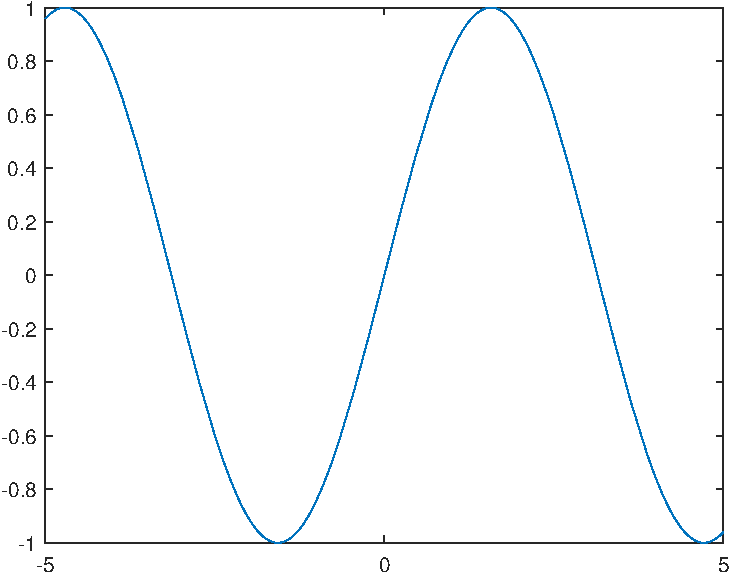
\includegraphics[width=0.9\textwidth]{image1}
% \caption{fig1}
% \label{fig:side:a}
% \end{minipage}%
% \begin{minipage}[t]{0.48\linewidth}
% \centering
% 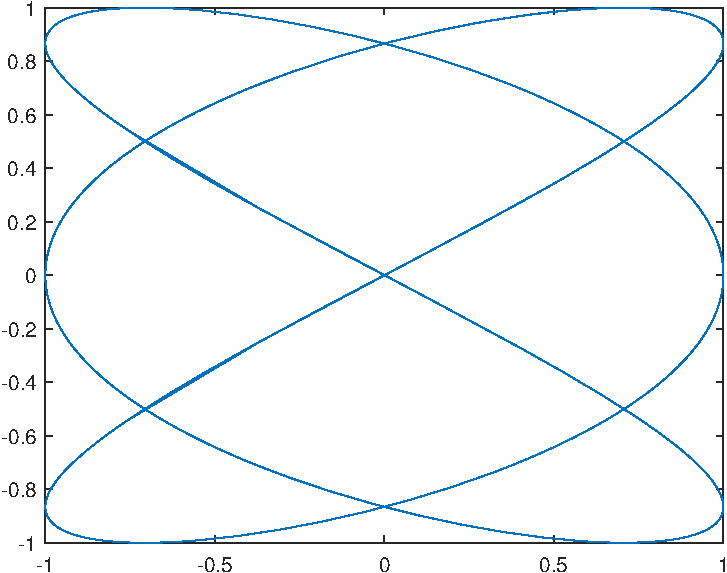
\includegraphics[width=0.9\textwidth]{image2}  % 2.2in
% \caption{fig2}
% \label{fig:side:b}
% \end{minipage}
% \end{figure}

% 这是一个算法流程图
% \begin{figure}[htp!]
% \centering
% 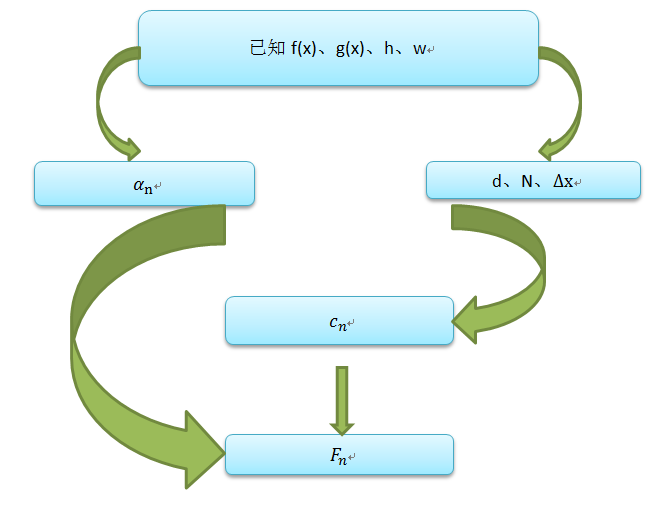
\includegraphics[width=.55\textwidth]{fig.png}
% \caption{算法流程图}
% \end{figure}

% 多图并排
% \begin{figure}[!htp]
% 	\centering
% 	\subfloat[Arabic numerals]{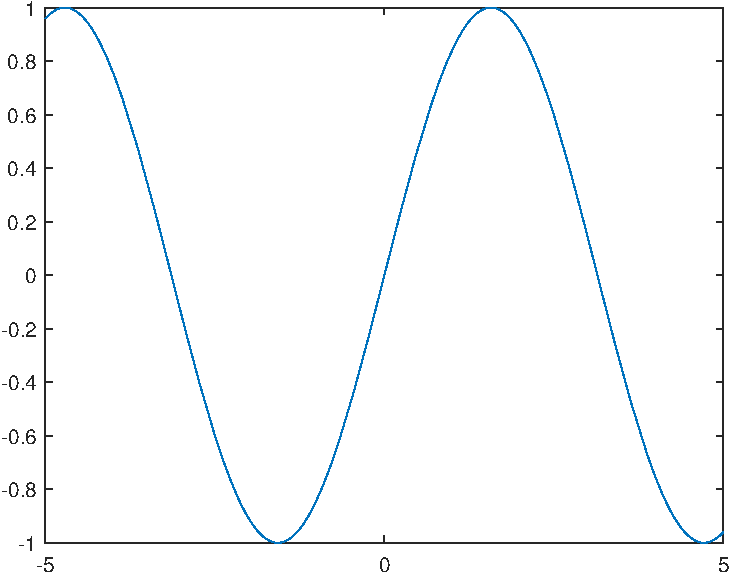
\includegraphics[width=0.4\textwidth]{image1}}\qquad
% 	\subfloat[Arabic numerals]{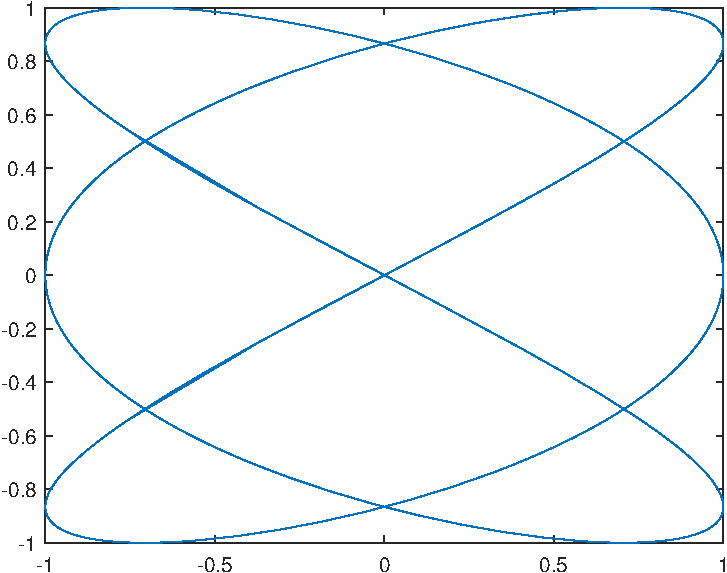
\includegraphics[width=0.4\textwidth]{image2}} \\
% 	\subfloat[Arabic numerals]{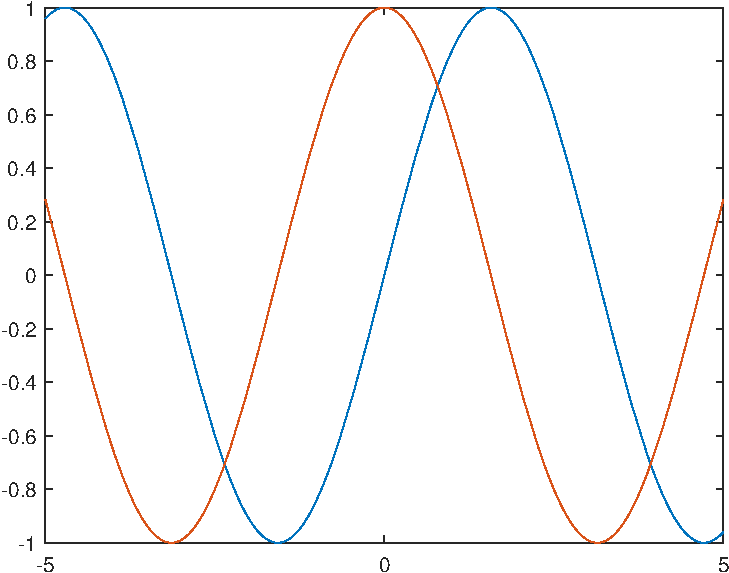
\includegraphics[width=0.4\textwidth]{image3}}\qquad
% 	\subfloat[Arabic numerals]{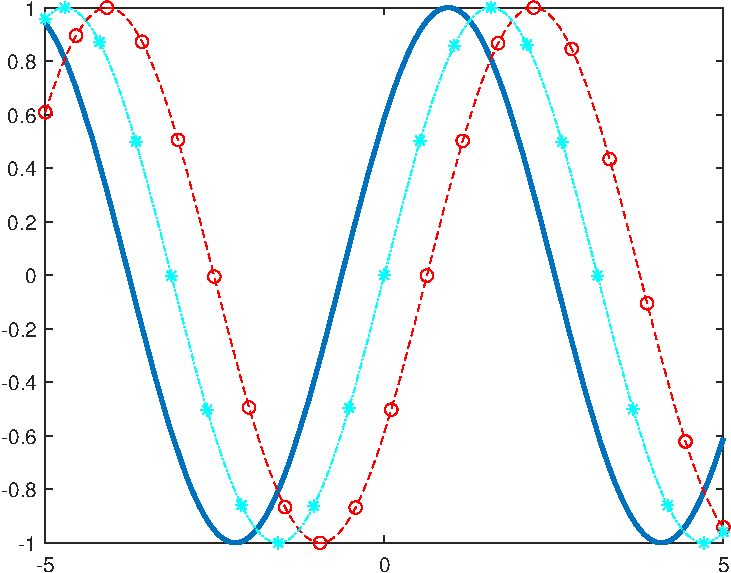
\includegraphics[width=0.4\textwidth]{image4}}
% 	\caption{多图示例}
% \end{figure}


% \clearpage
% \subsection{问题三分析}

% 题目要求制作软件的意思就是客户给定折叠桌高度、桌面边缘线的形状大小和桌脚边缘线的大致形状,将这些信息输入程序就得到客户想要的桌子。我们在求解最优设计加工参数时,自行给定桌面边缘线形状(椭圆、相交圆等),桌脚边缘线形状,折叠桌高度,应用第二问的非线性规划模型,用MATLAB软件绘制折叠桌截面图,得到自己设计的创意平板折叠桌。


% \section{模型评价}

% 这里是模型评价



% %参考文献   手工录入
% %\begin{thebibliography}{9}%宽度9
% % \bibitem{bib:one} ....
% % \bibitem{bib:two} ....
% %\end{thebibliography}

% %采用bibtex方案
% 这里引用第一篇文献\cite{rn1},第二篇文献\cite{rn2},第三篇文献\cite{rn3},第四篇专利\cite{rn4},以及第五篇文献\cite{rn5}。





% \clearpage
% %附录
% \begin{appendices}
% %\setcounter{page}{1} %如果需要可以自行重置页码。
% \section{MATLAB 源程序}
% \renewcommand{\thesubsection}{A\thinskip.\thinskip\arabic{subsection}}
% \subsection{第1问程序}
% \vspace{-2ex}

% \begin{Matlab}{code.m}
% clear all
% kk=2;
% [mdd,ndd]=size(dd);
% while ~isempty(V)
%     [tmpd,j]=min(W(i,V));
%     tmpj=V(j);
%     for k=2:ndd
%         [tmp1,jj]=min(dd(1,k)+W(dd(2,k),V));
%         tmp2=V(jj);
%         tt(k-1,:)=[tmp1,tmp2,jj];
%     end
%     tmp=[tmpd,tmpj,j;tt];
%     [tmp3,tmp4]=min(tmp(:,1));
%     if tmp3==tmpd,
%         ss(1:2,kk)=[i;tmp(tmp4,2)];
%     else
%         tmp5=find(ss(:,tmp4)~=0);
%         tmp6=length(tmp5);
%         if dd(2,tmp4)==ss(tmp6,tmp4)
%             ss(1:tmp6+1,kk)=[ss(tmp5,tmp4);tmp(tmp4,2)];
%         else, ss(1:3,kk)=[i;dd(2,tmp4);tmp(tmp4,2)];
%         end
%     end
%     dd=[dd,[tmp3;tmp(tmp4,2)]];
%     V(tmp(tmp4,3))=[];
%     [mdd,ndd]=size(dd);kk=kk+1;
% end;
% S=ss; D=dd(1,:);
% \end{Matlab}
% \vspace{2ex}

% \clearpage
% \section{Python 源程序}
% \renewcommand{\thesubsection}{B\thinskip.\thinskip\arabic{subsection}}
% \subsection{第2问程序}
% \vspace{-2ex}
% \begin{Python}{mip1.py}
% # This example formulates and solves the following  MIP model:
% #  maximize
% #        x +   y + 2 z
% #  subject to
% #        x + 2 y + 3 z <= 4
% #        x +   y       >= 1
% #        x, y, z binary

% # import gurobipy as gp
% from gurobipy import * #GRB
% try:
%     # Create a new model
%     m = Model("mip1")
%     # Create variables
%     x = m.addVar(vtype=GRB.BINARY, name="x")
%     y = m.addVar(vtype=GRB.BINARY, name="y")
%     z = m.addVar(vtype=GRB.BINARY, name="z")
%     # Set objective
%     m.setObjective(x + y + 2 * z, GRB.MAXIMIZE)
%     # Add constraint: x + 2 y + 3 z <= 4
%     m.addConstr(x + 2 * y + 3 * z <= 4, "c0")
%     # Add constraint: x + y >= 1
%     m.addConstr(x + y >= 1, "c1")
%     # Optimize model
%     m.optimize()
%     for v in m.getVars():
%         print('%s %g' % (v.varName, v.x))
%     print('Obj: %g' % m.objVal)

% except GurobiError as e:
%     print('Error code ' + str(e.errno) + ': ' + str(e))

% except AttributeError:
%     print('Encountered an attribute error')
% \end{Python}

% \end{appendices}



\end{document} 